\documentclass[11pt,french,A4paper,extrafontsizes,onecolumn,openright]{memoir}
\usepackage{lmodern}
\usepackage{amssymb,amsmath}
\usepackage{ifxetex,ifluatex}
\usepackage{fixltx2e} % provides \textsubscript
\ifnum 0\ifxetex 1\fi\ifluatex 1\fi=0 % if pdftex
  \usepackage[T1]{fontenc}
  \usepackage[utf8]{inputenc}
\else % if luatex or xelatex
  \ifxetex
    \usepackage{mathspec}
  \else
    \usepackage{fontspec}
  \fi
  \defaultfontfeatures{Ligatures=TeX,Scale=MatchLowercase}
\fi
% use upquote if available, for straight quotes in verbatim environments
\IfFileExists{upquote.sty}{\usepackage{upquote}}{}
% use microtype if available
\IfFileExists{microtype.sty}{%
\usepackage{microtype}
\UseMicrotypeSet[protrusion]{basicmath} % disable protrusion for tt fonts
}{}
\usepackage[margin=1in]{geometry}
\usepackage{hyperref}
\PassOptionsToPackage{usenames,dvipsnames}{color} % color is loaded by hyperref
\hypersetup{unicode=true,
            pdftitle={Trajectoires de biodiversité en forêt tropicale exploitée},
            pdfauthor={Ariane Mirabel},
            pdfkeywords={Biodiversity; Neotropical forests; Perturbation; Communities Ecology; Dynamic trajectories; Resilience},
            colorlinks=true,
            linkcolor=Maroon,
            citecolor=Blue,
            urlcolor=Blue,
            breaklinks=true}
\urlstyle{same}  % don't use monospace font for urls
\ifnum 0\ifxetex 1\fi\ifluatex 1\fi=0 % if pdftex
  \usepackage[shorthands=off,american,british,french,main=french]{babel}
\else
  \usepackage{polyglossia}
  \setmainlanguage[]{french}
  \setotherlanguage[variant=american]{english}
  \setotherlanguage[variant=british]{english}
  \setotherlanguage[]{french}
\fi
\usepackage{longtable,booktabs}
\usepackage{graphicx,grffile}
\makeatletter
\def\maxwidth{\ifdim\Gin@nat@width>\linewidth\linewidth\else\Gin@nat@width\fi}
\def\maxheight{\ifdim\Gin@nat@height>\textheight\textheight\else\Gin@nat@height\fi}
\makeatother
% Scale images if necessary, so that they will not overflow the page
% margins by default, and it is still possible to overwrite the defaults
% using explicit options in \includegraphics[width, height, ...]{}
\setkeys{Gin}{width=\maxwidth,height=\maxheight,keepaspectratio}
\IfFileExists{parskip.sty}{%
\usepackage{parskip}
}{% else
\setlength{\parindent}{0pt}
\setlength{\parskip}{6pt plus 2pt minus 1pt}
}
\setlength{\emergencystretch}{3em}  % prevent overfull lines
\providecommand{\tightlist}{%
  \setlength{\itemsep}{0pt}\setlength{\parskip}{0pt}}
\setcounter{secnumdepth}{5}
% Redefines (sub)paragraphs to behave more like sections
\ifx\paragraph\undefined\else
\let\oldparagraph\paragraph
\renewcommand{\paragraph}[1]{\oldparagraph{#1}\mbox{}}
\fi
\ifx\subparagraph\undefined\else
\let\oldsubparagraph\subparagraph
\renewcommand{\subparagraph}[1]{\oldsubparagraph{#1}\mbox{}}
\fi

%%% Use protect on footnotes to avoid problems with footnotes in titles
\let\rmarkdownfootnote\footnote%
\def\footnote{\protect\rmarkdownfootnote}

%%% Change title format to be more compact
\usepackage{titling}

% Create subtitle command for use in maketitle
\newcommand{\subtitle}[1]{
  \posttitle{
    \begin{center}\large#1\end{center}
    }
}

\setlength{\droptitle}{-2em}
  \title{Trajectoires de biodiversité en forêt tropicale exploitée}
  \pretitle{\vspace{\droptitle}\centering\huge}
  \posttitle{\par}
  \author{Ariane Mirabel}
  \preauthor{\centering\large\emph}
  \postauthor{\par}
  \predate{\centering\large\emph}
  \postdate{\par}
  \date{2018-06-28}


\begin{document}
\maketitle
\begin{abstract}
To be coming
\end{abstract}

{
\hypersetup{linkcolor=black}
\setcounter{tocdepth}{3}
\tableofcontents
}
\mainmatter

\chapter{Introduction générale}\label{introduction-generale}

\section{Les forêts tropicales humides, au coeur de l'avenir
planétaire}\label{les-forets-tropicales-humides-au-coeur-de-lavenir-planetaire}

Les forêts couvrent 30\% de la surface terrestre et les nombreux biens
et services environnementaux, économiques et sociaux qu'elles assurent
sont indispensables à l'équilibre planétaire. Elles régulent le climat,
la qualité de l'eau, de l'air et des sols et abritent une diversité
biologique exceptionnelle. Elles subviennent aux besoins alimentaires de
la population mondiale et permettent son développement économique en
tant que source de matières premières, de revenus et d'opportunités de
développement. Enfin, indispensables au bien être des populations, elles
représentent des valeurs historiques, culturelles et patrimoniales
irremplaçables (Forestry Department of the Food and Agriculture
Organization of the United Nations
\protect\hyperlink{ref-FRA2015}{2015}; Tilman, Isbell, et Cowles
\protect\hyperlink{ref-Tilman2014}{2014}). Malgré leur importance les
forêts restent extrêmement menacées par les changements climatiques
globaux, le traffic de bois illégal, la déforestation liée aux
changements d'usage des terres et les dégradations et pollutions
environnementales.

\subsection{Des écosystèmes
incontournables}\label{des-ecosystemes-incontournables}

Par ``forêt'' ou ``ecosystème forestier'' on entend les assemblages de
plantes, animaux et microorganismes et leur environnement qui
définissent une unité fonctionnelle dont les arbre sont les composants
essentiels (Forestry Department of the Food and Agriculture Organization
of the United Nations \protect\hyperlink{ref-FRA2000}{2000}). Ces
écosystèmes accueillent la diversité animale et végétale et les taux
d'endémismes les plus importants du globe et sont les régions restées
les moins anthropisées ce qui leur confère de forts enjeux de
conservation (Myers et al. \protect\hyperlink{ref-Myers2000}{2000};
Mittermeier et al. \protect\hyperlink{ref-Mittermeier2003}{2003}).

En entretenant les cycles de l'eau et des nutriments (azote, phosphore,
etc) via leur réseau racinaire, les forêts régulent la fertilité des
sols et les températures et les précipitations locales (Malhi et al.
\protect\hyperlink{ref-Malhi2008}{2008}; Isbell et al.
\protect\hyperlink{ref-Isbell2017}{2017}). Elles sont également des
puits de carbone qui représentent 1.1 ± 0.8 PgC.yr\textsuperscript{--1}
et jouent un rôle majeur dans la régulation des gaz à effet de serre
(\emph{GES}), d'une part en tant que puit de carbone qui compense les
émissions de GES mais également an tant que source potentielle lorsque
leur dégradation libère le carbone stocké dans leur biomasse (Pan et al.
\protect\hyperlink{ref-Pan2011}{2011}; Roy et Kumar
\protect\hyperlink{ref-Roy2017}{2017}).

A l'échelle globale la subsistance de 500 millions de personnes dépend
directement des forêts qui sont une source de biens allant de la
nourriture (par la chasse et la collecte de produits forestiers non
ligneux comestibles), à l'eau, aux matériaux de construction, et à
l'énergie (par l'utilisation du bois de chauffage et de cuisson des
aliments). L'exploitation forestière quant à elle représentait
\textasciitilde{} 1\% du PIB mondial, une part importante de l'emploi et
l'une des principales sources d'énergie en 2011 (Convention on
Biological Diversity et GmbH
\protect\hyperlink{ref-CBDdiversity2011}{2011}; FAO
\protect\hyperlink{ref-FAO2014}{2014}\protect\hyperlink{ref-FAO2014}{b}).

Enfin, les forêts interconnectées depuis toujours aux populations
humaines sont indispensables à leur bien être et ont une dimension
culturelle, spirituelle et patrimoniale importante.

\subsection{Des écosystèmes menacés, en particulier sous les
tropiques}\label{des-ecosystemes-menaces-en-particulier-sous-les-tropiques}

Bien qu'aussi indispensables qu'irremplaçables, les forêts disparaissent
et sont dégradées à une vitesse croissante: entre 2013 et 2015 leur
surface globale a ainsi diminué de 3\% (FAO
\protect\hyperlink{ref-FAO2009}{2014}\protect\hyperlink{ref-FAO2009}{a}).
Les forêts sont soumises à de fortes pressions anthropiques allant des
changements d'usage des terres, tels que le déboisement pour l'élevage
ou l'agriculture, à l'exploitation du bois légale ou illégale, à la
chasse ou à l'introduction d'espèces invasives. Elles subissent de plus
les changements climatiques globaux qui augmentent la fréquence des
événements extrêmes (sécheresses, incendies, inondations\ldots{})
(Pachauri et Meyer \protect\hyperlink{ref-Pachauri2014}{2014}).

Ces pressions diverses persistent voire s'accentuent malgré une prise de
conscience globale entérinée par la conférence des nations unies sur
l'environnement et le développement à Rio en 1992 qui a motivé de
nombreuses politiques de surveillance, de conservation de la
biodiversité et de préservation du fonctionnement des forêts (Summit
\protect\hyperlink{ref-Summit1992}{1992}; Schlaepfer et Elliott
\protect\hyperlink{ref-Schlaepfer2000}{2000}; Dirzo et Raven
\protect\hyperlink{ref-Dirzo2003a}{2003}; Morales-Hidalgo, Oswalt, et
Somanathan \protect\hyperlink{ref-Morales-Hidalgo2015}{2015}).

Ce contexte concerne en particulier les forêts tropicales, pour
lesquelles les menaces sont d'autant plus graves que leur importance au
niveau mondial est grande (Dirzo et Raven
\protect\hyperlink{ref-Dirzo2003a}{2003}; Hansen et al.
\protect\hyperlink{ref-Hansen2013}{2013}). Les bassins forestiers
tropicaux qui représentent 1.3 million d'hectares sont plus grandes
surfaces de forêts anciennes ``primaires'' n'ayant pas connu de forte
perturbation anthropique et accueillent la diversité biologique la plus
élevée au monde (Gentry \protect\hyperlink{ref-Gentry1988}{1988}; FAO
\protect\hyperlink{ref-FAO2011}{2011}). Historiquement peu peuplées, ces
régions connaissent une croissance démographique moyenne de près de
1,4\% par an qui entraîne des pressions anthropiques croissantes de
chasse, d'exploitation du bois, de conversion en terres agricoles et de
dégradation en forêts secondaires (Asner et al.
\protect\hyperlink{ref-Asner2009}{2009}).

Une attention particulière doit être portée aux zones tropicales pour
mieux comprendre leurs dynamiques et leur fonctionnement, toujours
partiellement méconnus aujourd'hui.

\subsection{La biodiversité: clé du fonctionnement des forêts
tropicales}\label{la-biodiversite-cle-du-fonctionnement-des-forets-tropicales}

La biodiversité n'est pas épargnée par les pressions globales actuelles
et une fraction significative est déjà anéantie et continue de
disparaître irréversiblement, si bien que l'on qualifie déjà cette
érosion croissantede sixième extinction de l'ère moderne (Vitousek et
al. \protect\hyperlink{ref-Vitousek1997}{1997}; Cardinale et al.
\protect\hyperlink{ref-Cardinale2012}{2012}).

La diversité des arbres, qui sont les éléments essentiels des
écosystèmes forestiers, détermine largement leur fonctionnement et
reflète celle autres groupes floristiques ou faunistiques (Guitet et al.
\protect\hyperlink{ref-Guitet2017}{2017}). Individuellement d'une part,
les espèces ont une valeur intrinsèque qui constitue le patrimoine
naturel global et selon leurs charactéristiques biologiques peuvent
avoir un rôle primordial, comme c'est le cas pour les espèces \emph{clé
de voûte}, (Jones, Lawton, et Shachak
\protect\hyperlink{ref-Jones1994}{1994}; Power et al.
\protect\hyperlink{ref-Power1996}{1996}; Gardner et al.
\protect\hyperlink{ref-Gardner2007}{2007}). D'autre part, la diversité
et la composition d'une communauté dans son ensemble définit la
complémentarité entre les individus qui la composent et l'utilisation et
la transformation des ressources. La diversité d'une communauté
détermine les flux d'eau, de nutriments et d'énergie à la base des
processus écosystémiques et donc sa productivité (Begon, Townsend, et
Harper \protect\hyperlink{ref-Begon2006}{2006}). Une diversité élevée
est de plus garante de la stabilité et la résilience des écosystèmes en
palliant l'impact des maladies, des espèces invasives et des variations
environnementales (Elmqvist et al.
\protect\hyperlink{ref-Elmqvist2003}{2003}).

On sait aujourd'hui que l'érosion de la biodiversité impacte le
fonctionnement des forêts mais les conséquences précises et la réponse
des écosystèmes dans le contexte actuel de changements globaux restent
mal connus. Pour avoir une comprendre et anticiper le devenir des forêts
dans le contexte actuel il est primordial de déterminer leurs dynamique
et leur réponse aux perturbation dans l'ensemble des aspects de leur
biodiversité.

\section{Les déterminants de la biodiversité: dynamique des communautés
et règles
d'assemblage}\label{les-determinants-de-la-biodiversite-dynamique-des-communautes-et-regles-dassemblage}

L'enjeu dans le contexte actuel est de prédire la réponse des
communautés aux perturbations en termes de diversité et de composition
et l'impact de ces changements sur leur fonctionnement des écosystèmes.
Comprendre et anticiper la réponse des peuplements revient à identifier
les processus écologiques qui régissent la dynamique des communautés et
qui déterminent la composition et la structure de la communauté à venir.

\subsection{Les règles d'assemblage des
espèces}\label{les-regles-dassemblage-des-especes}

La question fondamentale de l'écologie est de comprendre les processus
impliqués dans l'assemblage et la coexistence des espèces en
communautés. Plusieurs hypothèses sont débattues aujourd'hui, invoquant
soit des processus déterministes qui sélectionnent les espèces selon
leurs aptitudes dans l'environnement biotique et abiotique considéré
(Molino et Sabatier \protect\hyperlink{ref-Molino2001}{2001}), soit des
processus stochastiques relevant de la théorie neutre qui supposent un
assemblage dépendant uniquement de contraintes historiques et de
limitation de dispersion ou de croissance (Hubbell
\protect\hyperlink{ref-Hubbell2001}{2001}) \ref{fig:AssemblyRules}.

Ce débat sur les processus écologiques responsables de la structuration
des communautés est matérialisé dans le cas des forêts tropicales par la
controverse sur la théorie des perturbations intermédiaires
(\emph{Intermediaite Disturbance Hypothesis, IDH} en anglais). Cette
théorie prédit la prépondérance de processus déterministes d'exclusion
compétitive et de filtrage des espèces qui conduirait à une diversité
maximale pour un régime moyen de perturbations (Molino et Sabatier
\protect\hyperlink{ref-Molino2001}{2001}). Un tel régime de
perturbations modifierait régulièrement mais non drastiquement
l'environnment et créerait une variabilité constante dans l'espace et le
temps des conditions biotiques (interactions entre individus) et
abiotiques (ensoleillement, température, flux d'eau et de matière).
Cette variabilité permettrait à un large panel d'espèces de s'installer
soit parce que les conditions environnementales leur sont devenues
favorables soit parce qu'elles deviennent plus compétitives relativement
au reste de la communauté (Chesson
\protect\hyperlink{ref-Chesson2000}{2000}; Kariuki et al.
\protect\hyperlink{ref-Kariuki2006a}{2006}; Berry et al.
\protect\hyperlink{ref-Berry2008a}{2008}). A l'inverse la théorie neutre
suppose que les espèces sont équivalentes et que leur abondance ne
dépend pas de leurs caractéritiques écologiques et fonctionnelles mais
de processus aléatoires de dispersion, de croissance et de survie qui
résultent en un assemblage stochastique des communautés (Hubbell
\protect\hyperlink{ref-Hubbell2001}{2001}). Les deux hypothèses
déterministe et stochastique on démontré leur capacité à prédire la
structure des communautés à différentes échelles et à différents niveaux
de richesse. Ces hypothèses ce sont cependant pas incompatibles et il
est vraisemblable que les communautés réelles résultent de leur
actionconjointe selon une combinaison variable dans l'espace et le
temps. La question se porte alors sur l'importance relative de ces deux
processus neutres et déterministes et sur les facteurs qui les
influencent (Chave \protect\hyperlink{ref-Chave2004}{2004}).

\subsection{Mortalité et recrutement, moteurs de la dynamique des
communautés}\label{mortalite-et-recrutement-moteurs-de-la-dynamique-des-communautes}

La dynamique des communautés est constituée des processus démographiques
de mortalité (disparition), et de recrutement (apparition) des arbres
dans la communauté. Décomposer la dynamique des communautés selon ces
processus démographiques distingue leur importance respective dans le
maintien de l'écosystème et affine le rôle des processus d'assemblage
dans la réponse des communautés aux perturbations.

La mort d'un arbre provoque une trouée dans la canopée qui modifie
l'environnement abiotique (l'ensoleillement, les flux d'eau, de
nutriments et de matière) et l'environnement biotique (lesinteractions
entre individus), et impacte la croissance et l'établissement des arbres
environnants. La mortalité est un moteur essentiel de la dynamique des
communauté et de sa variabilité dans l'espace et le temps en tant que
processus aléatoire (Denslow, Ellison, et Sanford
\protect\hyperlink{ref-Denslow1998}{1998}; Sheil et Burslem
\protect\hyperlink{ref-Sheil2003}{2003}; Goulamoussène et al.
\protect\hyperlink{ref-Goulamoussene2017}{2017}; Otani et al.
\protect\hyperlink{ref-Otani2018}{2018}).

Le recrutement correspond à la suite d'événements biologiques allant de
la production, la dissémination et la germination des graines, à la
survie et la croissance des plantules jusqu'au seuil de recrutement. Ce
seuil correspond à un diamètre minimum, représentatif de la taille et de
la biomasse de l'arbre, à partir duquel l'individu est considéré comme
assez développé pour participer au fonctionnement de l'écosystème et
pour intégrer les inventaires. Le recrutement et les processus
écologiques dont il relève déterminent la dynamique et la structure des
commmunautés, en particulier après perturbation où leur résilience
dépend de la croissance des juvéniles et de la germination de graines du
sol (Denslow \protect\hyperlink{ref-Denslow1980}{1980}; Schnitzer et
Carson \protect\hyperlink{ref-Schnitzer2001}{2001}; Asner, Keller, et
Silva \protect\hyperlink{ref-Asner2004}{2004}).

\begin{figure*}

{\centering 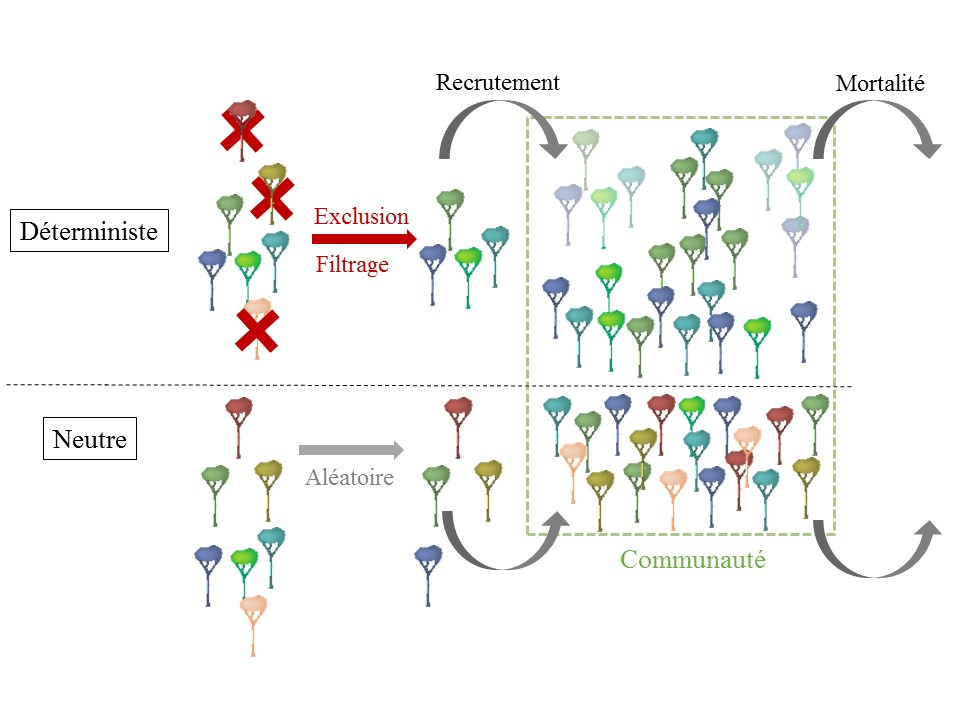
\includegraphics[width=1\linewidth]{ExternalFig/Fig_AssemblyRules} 

}

\caption{Schéma des processus déterminant la réponse des communautés végétales aux perturbations. Les processus déterministes (partie haute) sélectionnent les espèces recrutées dans la communauté selon leurs préférences environnementales e leur compétitivité, tandis que les processus stochastiques (partie basse) reviennent à une sélection aléatoire.}\label{fig:AssemblyRules}
\end{figure*}

\section{Comment mesurer la diversité biologique
?}\label{comment-mesurer-la-diversite-biologique}

Les processus démographiques et les règles d'assemblage d'espèces
déterminent la structure, la composition et la diversité des
communautés. Prédire et gérer l'avenir des forêts et en particularité de
leur précieuse diversité biologique nécessite de comprendre le rôle des
ces différents processus dans la définission de la diversité biologique
dans tous ses aspects. La biodiversité est définie de l'échelle du gène
à celle de l'écosystème considère la diversité des plantes, animaux,
champignons et microorganismes qui constituent les écosystèmes, de leur
variabilité génétique et phénotypique, et de la variabilité de leurs
assemblages (Loreau \protect\hyperlink{ref-Loreau2005}{2005}). La
biodiversité est souvent réduite à celle de richesse en espèces, mais
tient compte en réalité des multiples aspects de richesse,
d'homogenéité, de disparité et d'interactions entre les éléments du
vivant qui constituent les communautés. Appréhender les différents
aspects de la biodiversité permet d'identifier les mécanismes
écologiques fondamentaux qui régissent les écosystèmes et leurs
dynamiques spatiales et temporelles (Purvis et Hector
\protect\hyperlink{ref-Purvis2000}{2000}; Loreau
\protect\hyperlink{ref-Loreau2005}{2005}).

\subsection{Composition et dissimilarité entre
communautés}\label{composition-et-dissimilarite-entre-communautes}

De nombreuses mesures permettent d'estimer ce turnover, qui prennent en
compte ou non l'abondance des espèces (Podani, Ricotta, et Schmera
\protect\hyperlink{ref-Podani2013}{2013}). Nous avons choisis ici de
mesurer le taux de remplacement d'abondance, ou similarité de
Bray-Curtis, qui représente dans quelle mesure une communauté est le
sous-ensemble d'une plus grande. En pratique, si la communauté recrutée
après exploitation répond aux mêmes lois que la communauté initiale elle
sera équivalente à une communauté qui en aurait été tirée au hasard. La
similarité de Bray-Curtis mesure la somme des abondances d'une commaunté
remplacées par une espèce différente, normalisée par l'abondance totale
partagée entre les deux communautés \eqref{eq:formNestedness}.

\begin{equation}
T_{ab}=\frac{\sum_{i=1}^{n}|x_i^a - x_i^b| - \bigg| \sum_{i=1}^{n}{x_i^a} - \sum_{i=1}^{n}{x_i^b} \bigg|}{\sum_{i=1}^{n}\max{\left( x_i^a;x_i^b \right)}}
\label{eq:formNestedness}
\end{equation}

\subsection{Assemblage et structure des
communautés}\label{AbundanceDistribution}

Une communauté, qu'elle soit végétale, animale ou microbienne, est
constituée d'espèces aux effectifs différents: certaines sont très
abondantes, d'autres moyennement communes et d'autres encore, souvent la
majorité, sont rares. La façon la plus simple et immédiate de décrire
une communauté est de donner la distribution d'abondance de ses espèces,
qui représente les proportions d'espèces abondantes rapport aux espèces
communes ou rares. Cette distribution bien que variable d'une communauté
à l'autre, est régie par des lois écologiques lui donnant invariablement
une courbe en creux \ref{fig:AbdDist} (McGill et al.
\protect\hyperlink{ref-McGill2007}{2007}).

\begin{figure*}

{\centering 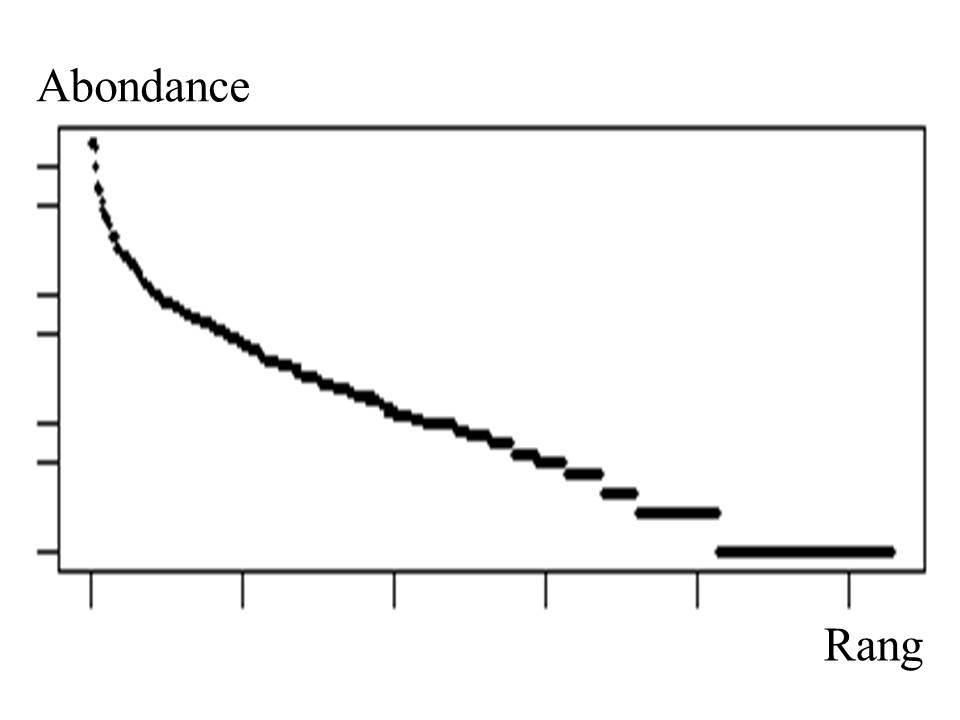
\includegraphics[width=0.6\linewidth]{ExternalFig/SpeciesAbdDist} 

}

\caption{Exemple de distribution d'abondance pour une communauté d'arbres en forêt tropicale humide}\label{fig:AbdDist}
\end{figure*}

Cette uniformité des distributions d'abondance a motivé le développement
de modèles proposant des relations mathématiques entre le nombre
d'espèces et leur abondance. Ces modèles reflètent le lien entre
l'importance d'une espèce dans la communauté et la quantité de
ressources qu'elle mobilise pour son développement: plus une espèce est
compétitive, plus elle sera abondante. Ce lien s'établit vis à vis de la
ressource limitante, qui peut être la lumière, l'eau disponible, les
nutriments du sol, l'espace, etc (Silvertown
\protect\hyperlink{ref-Silvertown2004}{2004}; Ter Steege et al.
\protect\hyperlink{ref-terSteege2006}{2006}). Prédire une distribution
d'abondance revient à prédire la répartition de la ressource limitante
entre les espèces de la communauté. De nombreux modèles prédictifs ont
été proposés, des modèles statistiques divisant aléatoirement la
ressource selon une loi de propabilité donnant les effectifs de chaque
espèce, aux modèles mécanistes divisant la resource selon une formule
prédéterminée, par exemple en la divisant successivement selon une
fraction constante (Fisher, Corbet, et Williams
\protect\hyperlink{ref-Fisher1943}{1943}; Motomura
\protect\hyperlink{ref-Motomura1932}{1932}; Tokeshi
\protect\hyperlink{ref-Tokeshi1993}{1993}; Magurran
\protect\hyperlink{ref-Magurran1988}{1988}).

Ces modèles testés pour de nombreuses communautés, ont démontré pouvoir
représenter correctement les communautés réelles et révéler les règles
écologiques qui en régissent l'assemblage. Ce sont des outils adéquats
pour comparer les communautés et en interpréter les différences, mais
manipuler une distribution d'abondance reste compliqué car il s'agit
d'une repréentation en 2D et ne permet pas de quantifier les différences
entre communautés. En revanche, les paramètres de ces distributions et
des modèle proposés pour les représenter permettent de quantifier le
nombre d'espèces, la forme des distribution, ou encore l'homogénéité des
abondances. Ces indicateurs sont les indices de diversité, résumant de
façon quantifiable les caractéristiques des distributions d'abondance.

\subsection{Les composantes de la
diversité}\label{les-composantes-de-la-diversite}

Si la biodiversité d'une communauté est souvent assimilée à sa richesse
en espèces, elle englobe en réalité le nombre, l'abondance, la
composition et les interactions entre les espèces. L'abondance en
particulier est essentielle: une espèce dominante n'apportera pas la
même contribution à l'écosystème qu'une espèce rare. Ainsi une
communauté dominée par une ou deux espèces très abondantes sera
intuitivement moins diverse qu'une autre avec autant d'espèces mais aux
abondances équivalentes. L'homogeneité des abondances dans une
population, ou \emph{équitabilité}, peut être bien plus révélatrice du
fonctionnement des écosystèmes que leur richesse ou leur composition.
Cette idée est illustrée par l'hypothèse du ratio de biomasse selon
laquelle les espèces dominantes sont bien plus déterminantes du
fonctionnement des écosystèmes que les espèces rares. Les espèces peu
communes n'ont une influence qu'à long terme, en tant que potentielles
futures espèces dominantes si l'environnement change, ou pas d'influence
si elles sont transitoires et ne persistent pas dans l'écosystème (Grime
\protect\hyperlink{ref-Grime1998}{1998}).

La richesse, simplement le nombre d'espèces recensées, et
l'équitabilité, la régularité de distribution d'abondance des espèces,
sont donc les deux composantes de la diversité taxonomique d'une
communauté \ref{fig:RichEqu} (Whittaker
\protect\hyperlink{ref-Whittaker1965}{1965}; Magurran
\protect\hyperlink{ref-Magurran2004}{2004}).

\begin{figure*}

{\centering 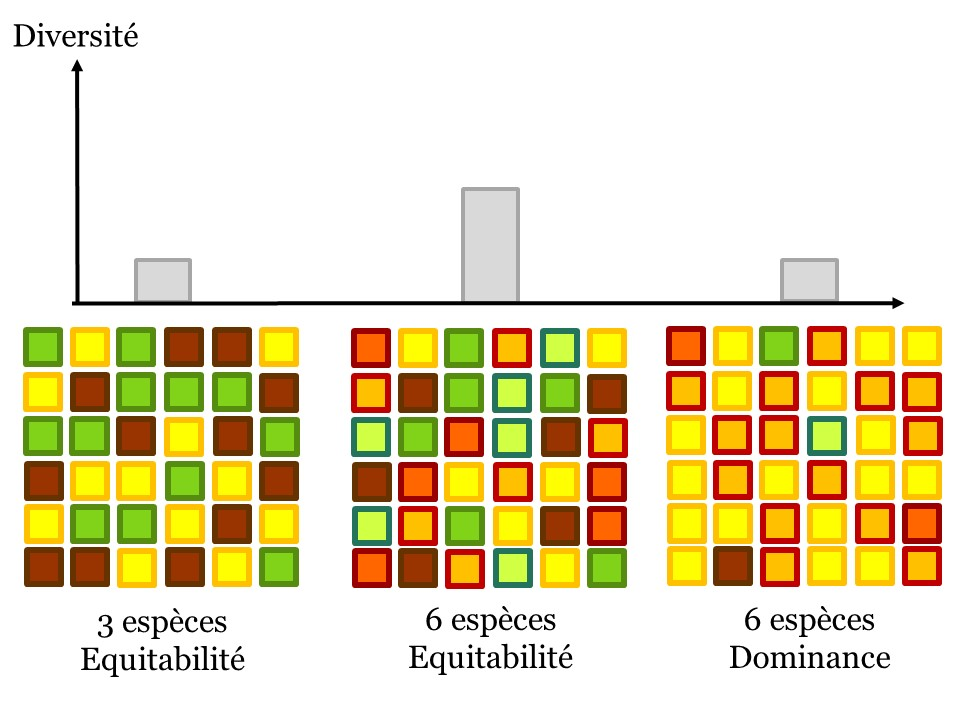
\includegraphics[width=0.6\linewidth]{ExternalFig/Fig_RichnessEquitability} 

}

\caption{Les deux composantes de la diversité taxonomique: richesse (nombre d'espèces) et équitabilité (homogeneité de répartition)}\label{fig:RichEqu}
\end{figure*}

Mesurer la diversité ne revient donc pas à une mesure unique mais
plusieurs indices de diversité qui combinent différemment les
composantes de la diversité. Plusieurs familles d'indices de diversité
ont été développées et regroupent les indices mesurés selon une même
formule dont les déclinaisons accordent un poids variables aux
composantes de la diversité. La famille des indices de diversité de
Réyni par exemple, judicieuse pour l'étude des communautés végétales,
rassemble les indices mesurés selon l'équation \eqref{eq:formHCDT} modulée
par un paramètre \emph{q} appelé ``ordre de diversité'' qui correspond
au poids des espèces rares par rapport aux espèces abondantes (Mendes et
al. \protect\hyperlink{ref-Mendes2008}{2008}). Plus l'ordre de diversité
est élevé, plus les espèces rares sont négligées par rapport aux espèces
abondantes.

\begin{equation}
{^{q}H=\frac{1}{q-1}\Bigg(1-\displaystyle\sum_{s=1}^{S}p^q_s\Bigg) }
\label{eq:formHCDT}
\end{equation}

Dans cette famille d'indices de diversité se retrouvent les indices les
plus utilisés dans la littérature: l'ordre 0 où chaque espèce contribue
de la même façon correspond à la richesse spécifique, l'ordre 1 où
richesse et équitabilité sont également prises en compte correspond à
l'indice de Shannon, et l'ordre 2 pour lequel les espèces rares sont
presque négligées correspond à l'indice de Simpson (parfois appelé
``diversité en espèces abondantes'') (Shannon
\protect\hyperlink{ref-Shannon1948}{1948}; Simpson
\protect\hyperlink{ref-Simpson1949}{1949}; Patil et C.
\protect\hyperlink{ref-Patil1982}{1982}; Tothmeresz et Tóthmérész
\protect\hyperlink{ref-Tothmeresz1995}{1995}).

Ces indices, mathématiquement corrects et représentatifs des différentes
composantes de la diversité, ne donnent cependant pas un nombre
intelligible qui permettent de comparer facilement différentes
communautés. Les indices de diversité doivent être traduits en
\emph{nombre équivalent d'espèces} qui correspond au nombre d'espèces
qu'aurait la communauté étudiée si toutes les espèces avaient la même
abondance. Ce nombre équivalent d'espèces, ou \emph{nombre de Hill}, est
obtenu par transformation des valeurs obtenues par une exponentielle à
base q (Hill \protect\hyperlink{ref-Hill1973}{1973}).

Les mesures de diversité choisies sont donc la traduction intelligible
en nombre équivalent d'espèces d'une déclinaison d'indices combinant
richesse et équitabilité de différentes façons pour capter toute
structure de diversité.

\subsection{Résolution du biais
d'échantillonnage}\label{resolution-du-biais-dechantillonnage}

En pratique aucun inventaire n'est exhaustif et l'étude de la diversité
se heurte aux biais d'échantillonnage qui sous-estiment la richesse et
faussent l'abondance des espèces. Corriger ce biais nécessite d'estimer
les abondances réelles à partir des observations et des relations
mathématiques reliant les abondances des différentes espèces. La
première méthode développée correspond à la formule des fréquences de
Turing (Good \protect\hyperlink{ref-Good1953}{1953}) où l'abondance
réelle *\alpha\_v* d'une espèce observée \emph{v} fois dans un
échantillonnage de \emph{n} individus dépend du nombre d'espèces
observées également \emph{v} fois et d'e celles'espèces observées
\emph{v+1} fois @ref\{eq=formGoodTuring\}:

\begin{equation}
\alpha_v=\frac{\big(v+1\big)}{n}\frac{s^n_{v+1}}{s^n_v}
\label{eq:formGoodTuring}
\end{equation}

Les singletons (espèces observées une seule fois) et les doubletons
(espèces observées deux fois) sont alors particulièrement intéressants
car il permettent d'estimer le nombre \emph{s\^{}n\_0} d'espèces
observées zéro fois (\(s^n_0=\frac{s^n_1}{n}\)) qui ont été manquées
dans l'inventaire et peuvent être ajoutées aux observation pour corriger
le biais d'échantillonnage de la richesse.

De nombreuses méthodes ont repris cette relation en y intégrant
notamment la notion de \emph{taux de couverture} qui quantifie l'effort
d'échantillonnage d'un inventaire réel et permet de savoir quelle
proportion de la communauté est échantillonnée (Dauby et Hardy
\protect\hyperlink{ref-Dauby2012}{2012}). La correction la plus adéquate
a pu être déterminée selon le taux de couverture de l'inventaire et les
estimateurs de la diversité sont aujourd'hui très fiables (Chao et Jost
\protect\hyperlink{ref-Chao2015}{2015}; Marcon
\protect\hyperlink{ref-Marcon2015b}{2015}).

\subsection{Diversité fonctionnelle}\label{diversite-fonctionnelle}

Les mesures de diversité décrites précédemment, appelées diversité
neutre, considèrent toutes les espèces de la même façon que celles-ci
aient ou non des caractéristiques biologiques ou phylogénétiques
proches. Ces diversités peuvent cependant facilement intégrer les
caractéristiques des espèces en mesurant leur similarité et une
communauté sera d'autant plus diverse que les espèces qui la constituent
sont différentes. Pour des communautés végétales la diversité
phylogénétique considère les distances entre espèces dans un arbre
phylogénétique et la diversité fonctionnelle considère leurs différences
morphologiques ou physiologiques \ref{fig:RichEquSim}.

\begin{figure*}

{\centering 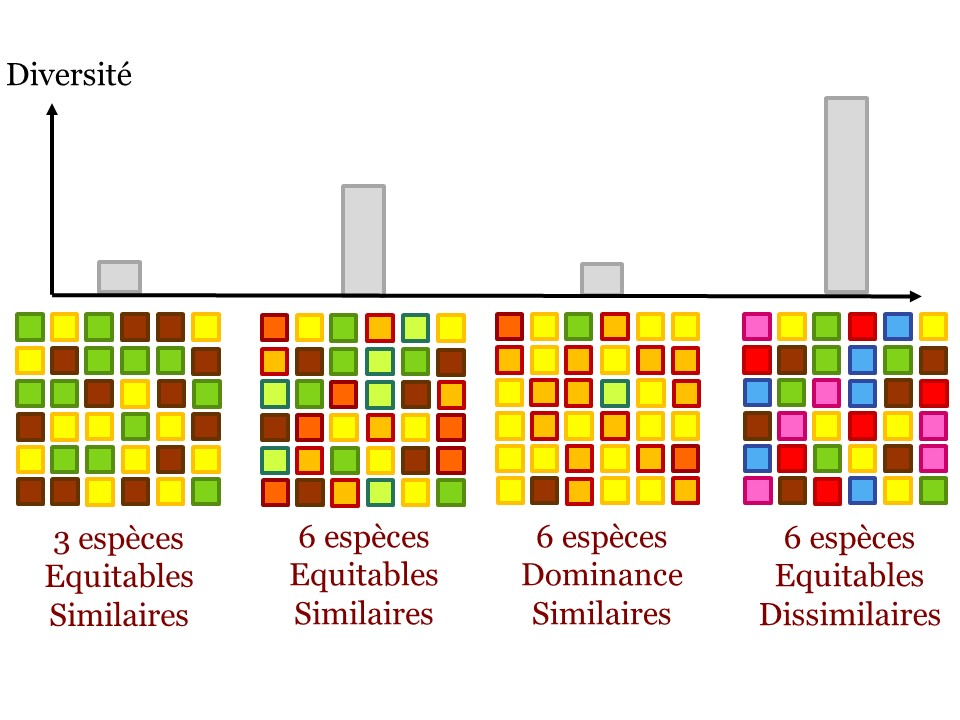
\includegraphics[width=0.6\linewidth]{ExternalFig/Fig_RichnessEquitabilitySimilarity} 

}

\caption{Troisième composante de la diversité: la similarité entre espèces basée sur des distances phylogénétiques ou taxonomiques}\label{fig:RichEquSim}
\end{figure*}

Ces similarités sont ensuite intégrées aux indices de diversité, au même
titre que la richesse et l'équitabilité, sous la forme d'une matrice de
distances entre espèces calculée sur la base de leur phylogénie ou de
leurs traits fonctionnels.

Les traits fonctionnels sont les caractéristiques morphologiques,
physiologiques et phénologiques des espèces, ils déterminent le
fonctionnement des individus, leur performance de croissance et de
survie, et leurs interaction avec l'environnement (Violle et al.
\protect\hyperlink{ref-Violle2007b}{2007}). L'approche fonctionnelle
décrivant les espèces et les individus selon leurs caractéristiques
biologiques a été largement adoptée en écologie. D'une part, cette
approche réduit la dimensionnalité des communautés, indispensable pour
l'étude d'écosystèmes aussi riches que les forêts tropicales et permet
de comparer les communautés quelle que soit leur composition en espèces
(Begon, Townsend, et Harper \protect\hyperlink{ref-Begon2006}{2006};
Scheiter, Langan, et Higgins \protect\hyperlink{ref-Scheiter2013}{2013};
Mouillot et al. \protect\hyperlink{ref-Mouillot2013a}{2013}; Sakschewski
et al. \protect\hyperlink{ref-Sakschewski2016}{2016}). D'autre part,
composition et diversité fonctionnelle sont interprétables en termes
d'utilisation des ressources et de flux de matière et d'énergie, et
relient directement la diversité des communautés à leur fonctionnement.
Enfin, cette approche appréhende la signature fonctionnelle des
perturbations et permet d'identifier et de quantifier les processus
déterminant la dynamique des communautés (Funk et al.
\protect\hyperlink{ref-Funk2017}{2017}). La définition des processus
déterministes est qu'ils n'impliquent pas les espèces de la même façon
selon leurs caractéristiques biologiques: l'exclusion abiotique
d'espèces non adaptées à l'environnement se traduiront par une
aggrégation de la communauté dans l'espace des traits fonctionnels et
une diminution de sa diversité fonctionnelle, tandis que l'exclusion
compétitive limitant les similarité entre espèces se traduira par une
dispersion des traits fonctionnels de la communauté et une diversité
fonctionnelle élevée (McGill et al.
\protect\hyperlink{ref-McGill2006}{2006}; Kunstler et al.
\protect\hyperlink{ref-Kunstler2012}{2012}).

L'approche fonctionnelle nécessite de choisir judicieusement les traits
intégrés aux indices de diversité. Une vaste littérature a permis
d'identifier les traits clés représentatifs de l'écologie et de la
croissance des espèces et de leur influence sur le fonctionnement de
l'écosystème (Reich \protect\hyperlink{ref-Reich2014}{2014}). Les traits
foliaires tout d'abord, qui déterminent la stratégie d'acquisition et
d'allocation des resources lumineuses, définissent un ``spectre
économique foliaire'' qui oppose les espèces à larges feuilles fines
ayant une forte capacité photosynthétique permettant une acquisition
rapide des resources, aux espèces à petites feuilles coriaces et
résistantes. Un gradient similaire s'applique aux traits racinaires et
aux propriétés du bois, opposant les espèces aux tissus légers à courte
durée de vie permettant une croissance rapide à celles aux tissus denses
plus résistants et mobilisant plus de ressources (Chave et al.
\protect\hyperlink{ref-Chave2009}{2009}; Valverde-Barrantes et al.
\protect\hyperlink{ref-Valverde-Barrantes2017}{2017}). Les stratégies
d'acquisition des resources déterminent la stratégie de croissance des
espèces: les espèces ``acquisitives'' auront une croissance rapide et
une courte durée de vie tandis que les espèces ``conservatives'' auront
une croissance plus lente mais une meilleure résistance aux conditions
environnementales éprouvantes (Reich, Walters, et Ellsworth
\protect\hyperlink{ref-Reich1997}{1997}; Wright et al.
\protect\hyperlink{ref-Wright2004}{2004}). A ces traits fonctionnels
mesurables à l'échelle de l'individus s'ajoutent des \emph{traits
d'histoire de vie} mesurables à l'échelle de l'espèce. Parmi ces traits
la masse des graines et la hauteur moyenne maximale des arbres à l'âge
adulte ont montré être particulièrement représentatifs des stratégies de
croissance, de survie et de reproduction (Westoby
\protect\hyperlink{ref-Westoby1998}{1998}; Hérault et al.
\protect\hyperlink{ref-Herault2011}{2011}). La combinaison de l'ensemble
de ces traits spécifique, foliaires, racinaires et du bois appréhende la
stratégie fonctionnelle des espèces, leurs préférences écologiques et
leur performance de croissance et de survie. L'engouement récent de
l'écologie pour l'approche fonctionnelle a de plus permis la création de
bases de données fonctionnelles conséquentes et standardisées qui
rendent possibles l'approche fonctionnelle à l'échelle des communautés
{[}Kattge et al. (\protect\hyperlink{ref-Kattge2011}{2011});
Pérez-Harguindeguy et al.
(\protect\hyperlink{ref-Perez-Harguindeguy2013}{2013});\footnote{\url{http://www.ecofog.gf/Bridge/}}{]}

L'approche fonctionnelle considère la diversité des communautés mais
également leur composition fonctionnelle mesurable par les valeurs
moyennes de traits pondérées par l'abondance des espèces
(\emph{Community Weighted Means, CWM} en anglais). L'abondance des
caractéristiques fonctionnelles détermine à la fois le fonctionnement
des communautés et leur résilience. D'après la théorie du ``ratio de
biomasse'' (Grime \protect\hyperlink{ref-Grime1998}{1998}), le rôle d'un
individu dans l'écosystème dépend de la fraction de biomasse qu'il
représente et le fonctionnement des communautés repose sur les espèces
dominantes tandis que les espèces rares ont peu d'influence.

Par ailleurs la répartition d'abondance des traits fonctionnels amène à
la notion de redondance fonctionnelle qui quantifie le nombre d'espèces
partageant les mêmes valeurs de traits. La redondance fonctionnelle,
souvent élevée en forêt tropicale, permet aux communautés de perdre des
espèces sans nécessairement voir disparaître leur rôle dans
l'écosystème: la redondance détermine en partie la résilience des
communautés et atténue l'impact des perturbations. L'organisation de la
redondance dans l'espace des traits d'une communauté renseigne sur les
assemblages les plus stables qui se dégageraient le plus probablement
après de nouvelles perturbations. La redondance fonctionnelle d'une
communauté peut se mesurer dans l'espace fonctionnel à partir de la
densité de probabilité de traits (\emph{Traits Density Probability, TDP}
en anglais) de chaque espèce (Carmona et al.
\protect\hyperlink{ref-Carmona2016}{2016}). Les densités des espèces
d'une communauté pondérées par leur abondance sont additionnées pour
donner la redondance fonctionnelle sur l'ensemble de l'espace
fonctionnel ou sur un espace restreint, comme nous le ferons par la
suite quand on s'intéressera à la redondance fonctionnelle dans l'espace
de la communauté de départ \ref{fig:RedundancyMethod}.

\begin{figure*}

{\centering 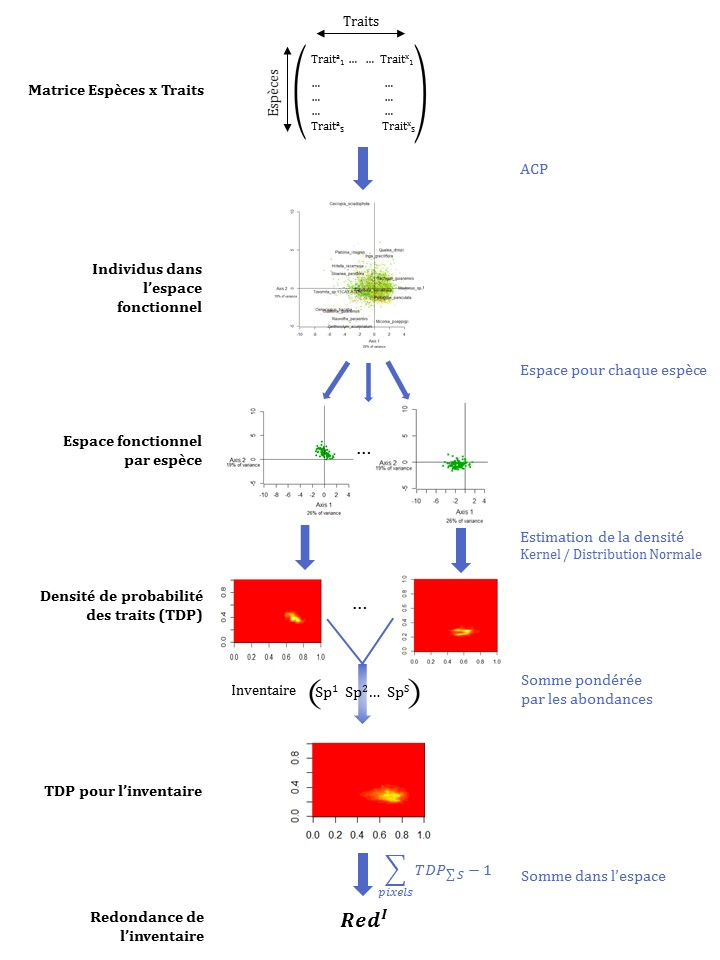
\includegraphics[width=1\linewidth]{ExternalFig/Fig_MesureRedondance} 

}

\caption{La redondance fonctionnelle est la somme des chevauchement entre espèces dans l'espace fonctionnel. Les individus de la base de données fonctionnelle sont représentés dans un espace à 2 dimensions grâce à une analyse en composantes principales (ACP). Une estimation par noyau estime ensuite la densité de probabilité des traits (TDP) de chaque espèce. La somme de ces densités pondérées par l'abondance des espèces donne enfin la redondance fonctionnelle de la communauté, interprétable comme le nombre d'espèces qui peuvent disparaître sans diminuer l'espace fonctionnel de la communauté.}\label{fig:RedundancyMethod}
\end{figure*}

\section{La Guyane Française et l'exemple de la station de
Paracou}\label{la-guyane-francaise-et-lexemple-de-la-station-de-paracou}

Le bassin Amazonien est la plus riche des trois principales régions de
forêt tropicale humide (Gentry \protect\hyperlink{ref-Gentry1988}{1988})
et la Guyane française en est une région de 83 846 km\textsuperscript{2}
recouverte à 95\% forestière au Nord-Est du continent sud-américain
entre le Surinam et le Brésil.

\subsection{Le contexte Guyanais}\label{le-contexte-guyanais}

La région appartient au bouclier des Guyanes qui s'étend de l'Amapa au
Brésil jusqu'au delta de l'Orénoque au Venezuela. Formé il y a plus de 2
milliards d'années, le bouclier des Guyanes est un assemblage d'unités
géomorphologiques façonnées par une succession d'épisodes géologiques,
climatiques et marins. Ces unités correspondent à des conditions
pédologiques, climatiques et topographiques déterminant la composition
et la diversité du couvert végétal et les processus écologiques qui les
régissent, tels que les migrations et le filtrage environnemental
(Guitet et al. \protect\hyperlink{ref-Guitet2015}{2015}).

Le relief Guyanais est une grande diversité topographique qui alterne
entre des collines allant jusqu'à 50m d'altitude, et des bas-fonds
humides. Les sols sont des Acrisols recouvrant une couche de saprolite
transformée peu perméable qui entraîne un drainage latéral des
précipitations. La profondeur des sols, leur composition et leur
capacité de rétention et de drainage de l'eau sont très hétérogènes
(Ferry et al. \protect\hyperlink{ref-Ferry2010}{2010}; Robert et Moravie
\protect\hyperlink{ref-Robert2003}{2003}).

Le climat est un climat tropical humide, davantage marqué par le régime
des précipitations que par celui des températures. La température
moyenne est 26°C et reste constante au cours de l'année tandis les
précipitations moyennes annuelles varient de 2 000 à 4 000
mm.an\textsuperscript{-1} et montrent une grande variabilité spatiale et
temporelle. Les précitations suivent un gradient décroissant marqué
d'est en ouest et une forte variabilité au cours de l'année, avec une
saison humide entre novembre et avril et une saison sèche d'avril à
mi-juillet durant laquelle les précipitations sont inférieures à 50 mm
(Wagner et al. \protect\hyperlink{ref-Wagner2011}{2011}).

La forêt Guyanaise est une forêt équatoriale sempervirente ombrophile de
plaine. D'une richesse incroyable, elle accueille plus de 7 000 espèces
végétales (hors champignons) dont 1 500 espèces d'arbres et une richesse
faunistique toute aussi incroyable (Noter
\protect\hyperlink{ref-DeNoter2008}{2008}). La composition taxonomique
des arbres est très variable sur le territoire. Plusieurs patrons de
composition on été mis en évidence selon un gradient du nord-ouest où
dominent les familles botaniques des \emph{Lecythidaceae} et
\emph{Cesalpinaceae}, au sud-est où dominent \emph{Burseraceae} et
\emph{Mimosaceae}. Ces patrons suivent en particulier par une
combinaison de gradients topographique et pédologique (Sabatier et
Prévost \protect\hyperlink{ref-Sabatier1989}{1989}; Sabatier et al.
\protect\hyperlink{ref-Sabatier1997}{1997} cf Toto; Guitet et al.
\protect\hyperlink{ref-Guitet2015}{2015}).

\subsection{Paracou, plus de 30 de suivi de la forêt
Amazonienne}\label{paracou-plus-de-30-de-suivi-de-la-foret-amazonienne}

Le dispositif de Paracou, installé entre les communes de Kourou et
Sinnamary (5°18'N and 52°53'W), a été mis en place en 1984 pour étudier
l'impact de l'exploitation forestière sélective sur les peuplements
forestiers. Le dispositif correspond à l'origine à 12 parcelles de 6.25
ha ayant subi en 1984 un gradient de trois intensités d'abattage,
d'éclairices et de coupe de bois de chauffage. Le traitement de
perturbation a été attribué selon un dispositif aléatoire de trois
réplications de 4 traitements: parcelles témoins sans intervention
(\emph{T0}), traitement 1 avec coupes d'abattage (\emph{T1}), traitement
2 avec abattage et éclaircies par annélation (\emph{T2}), traitement 3
avec abattage, éclaircies et coupe de bois de chauffage (\emph{T3})
\ref{tab:InterventionTable}.

En 1990, trois parcelles de 6.25ha et une parcelle de 25ha (parcelles
13, 14, 15 et 16) ont été ajoutées au dispositif pour l'étude et le
suivi de la diversité en forêt non perturbée \ref{fig:ParacouDesign}.

\begin{figure*}

{\centering \includegraphics[width=0.6\linewidth]{ExternalFig/Paracou} 

}

\caption{Dispositif expérimental de Paracou, schéma des 16 parcelles de suivi des dynamiques forestières. La couleur des parcelles indique l'intensité de perturbation appliquée à 9 des parcelles en 1984 (voir le tableau 1.}\label{fig:ParacouDesign}
\end{figure*}

Sur l'ensemble du dispositif sont recensées 591 espèces d'arbres
appartenant à 223 genre et 64 familles botaniques, principalement les
\emph{Fabaceae}, les \emph{Chrisobalanaceae}, les \emph{Lecythidaceae}
et les \emph{Sapotaceae}. Les températures annuelles atteignent 26°C et
les précipitations 2 980 mm.an\textsuperscript{-1} de mi-août à
mi-novembre, avec une saison sèche d'un mois en mars (Wagner et al.
\protect\hyperlink{ref-Wagner2011}{2011}).

\subsection{Méthodes d'inventaires}\label{methodes-dinventaires}

Depuis la mise en place du dispositif en 1984 toutes les parcelles sont
inventoriées chaque année à la saison sèche à partir de mi-juillet. Tous
les arbres de plus de 10 cm de diamètre à 1.30 m (diamètre à hauteur de
poitrine, \emph{DBH} en anglais) sont identifiés, numérotés et
cartographiés. Les arbres morts sont relevés chaque année et notés en
précisant le type mort (mort sur pied, chablis primaire ou chablis
secondaire).

Lorsqu'un arbre atteint 10 cm il est \emph{recruté} et sera mesuré
chaque année. Il est identifié dans un premier temps par un nom
\emph{vernaculaire}, ou nom commun, attribué par l'équipe de terrain. En
1984, 62 espèces commerciales étaient identifiées par un nom commun
propre tandis que toutes les autres espèces étaient regroupées sous deux
noms vernaculaires distinguant les palmiers des espèces arborées. Cette
identification en nom vernaculaire s'est précisée par la suite et
aujourd'hui 235 noms vernaculaires différents sont recensés pour
l'ensemble du dispositif sur les 30 ans de suivi. Des campagnes
d'identification botanique au cours desquelles les arbres sont
identifiés au niveau espèce botanique ont été mises en place à partir de
2003 et se poursuivent depuis tous les 5 à 6 ans.

L'histoire des inventaires botaniques s'étant construite petit à petit
au gré des nouveaux projets et des forces en présence, la précision et
le taux d'identification botaniques sont variables au cours du temps et
entre les parcelles. Ceci génère des incertitudes taxonomiques
importantes, les noms vernaculaires correspondant souvent à plusieurs
noms botaniques et inversement (Oldeman
\protect\hyperlink{ref-Oldeman1968}{1968}). Le soucis vient alors des
arbres n'ayant qu'un identification en nom vernaculair, lorsque
l'individu est mort avant d'avoir pu être identifié au cours d'une
campagne botanique par exemple.

\section{Problématique et plan de la
thèse}\label{problematique-et-plan-de-la-these}

La thèse présentée ici cherche à déterminer la réponse aux perturbations
d'une forêt tropicale naturelle en termes de diversité taxonomique et
fonctionnelle, à en interpréter les processus sous-jacents et à
clarifier la résilience des forêts tropicales dans le contexte des
changements actuel. Le document s'organise en trois chapitres
correspondant à trois articles scientifiques en cours de rédaction (pour
le moment!).

\begin{itemize}
\item
  Le premier chapitre présente une méthode de propagation des
  incertitudes taxonomiques permettant d'estimer la diversité des
  communautés en résolvant le problème des indéterminations botaniques.
  La méthode se base sur la reconstitution d'inventaires complets
  théoriques à partir des associations entre noms vernaculaires et
  botaniques. Dans un premier temps nous calibrons la méthode de façon à
  avoir une estimation de la diversité la plus précise possible. Dans un
  deuxième temps nous appliquons la méthode de propagation au cas des
  inventaires forestiers réels, qui sont une large et précieuse source
  d'information, et proposons une méthode d'inventaires optimisée pour
  une estimation précise de la diversité. Nous proposons enfin
  l'application de cette méthode aux dispositifs expérimentaux, dont les
  contraintes d'identification sont différentes, et qui sera utilisée
  dans la suite de ce travail.
\item
  Dans le deuxième chapitre nous avons étudier les trajectoires de
  composition et de diversité taxonomique et fonctionnelle des parcelles
  de Paracou. Ces trajectoires permettent de clarifier l'impact des
  perturbations sur la structure des communautés, d'identifier les
  processus écologiques sous-jacents et d'évaluer la résilience des
  communautés. En particulier, nous examinons les trajectoires
  taxonomiques et fonctionnelles et leurs implications pour le
  fonctionnement et la résilience de l'écosystème. Nous testons la
  validité de la théorie des perturbations intermédiaires, débattue en
  forêt tropicale et rarement testée sur le long terme. Enfin, nous
  concluons sur les différents aspects de la résilience des communautés
  et leurs implications pour la gestion des forêts tropicales.
\item
  Dans le troisième chapitre nous étudions spécifiquement les
  trajectoies du recrutement qui permettent de préciser l'impact de la
  perturbation sur les processus démographiques et écologiques qui
  structurent les communautés. Ces trajetoires permettent d'identifier
  les phases successives de recrutement après exploitation, d'en décrire
  les processus écologiques sous-jacents et de mieux appréhender la
  résilience de la communauté et des processus qui la maintiennent, et
  d'anticiper la réponse à de nouvelles perturbations.
\end{itemize}

\chapter{Article 1 : Des inventaires forestiers aux trajectoires de
diversité: le problème universel de
l'incertitude}\label{article-1-des-inventaires-forestiers-aux-trajectoires-de-diversite-le-probleme-universel-de-lincertitude}

Malgré les enjeux liés aux forêts tropicales et l'urgence d'en préserver
l'intégrité et le fonctionnement, seule une petite fraction de leur
diversité est connue. Le nombre d'espèces inventoriées sous les
tropiques ne correspondant qu'à une observation unique (Feeley et Silman
\protect\hyperlink{ref-Feeley2011}{2011}) présume de l'ampleur de notre
méconnaissance et rend impossible toute supposition sur la distribution
des espèces et leurs dynamiques. Il est essentiel d'améliorer notre
connaissance du vivant, en fournissant un plus grand effort
d'échantillonnage et en valorisant toute connaissance déjà disponible.

Le coût des inventaires en temps, en main d'oeuvre et en moyens,
d'autant plus important que le niveau de l'inventaire est précis,
implique de travailler également à des méthodes pour valoriser tout type
d'inventaires (Baraloto et al.
\protect\hyperlink{ref-Baraloto2012}{2012}). Dans le cas de l'étude des
peuplements forestiers, les inventaires d'exploitation peu coûteux et
couvrant des surfaces larges sont une source d'information
incontournable (Ter Steege et al.
\protect\hyperlink{ref-terSteege2000}{2000}; Guitet et al.
\protect\hyperlink{ref-Guitet2014}{2014}).

\section{Noms vernaculaires et propagation des incertitudes
taxonomiques}\label{noms-vernaculaires-et-propagation-des-incertitudes-taxonomiques}

Ces inventaires ne sont cependant généralement pas réalisés en noms
scientifiques mais noms vernaculaires, qui sont mieux connus, plus
faciles à attribuer car basés sur des critères morphologiques, culturels
ou d'usage et qui ne nécessitent pas de vérification botanique
ultérieure à partir d'herbiers. Cette simplicité se fait cependant au
détriment de la fiabilité des noms vernaculaires, qui correspondent à
plusieurs espèces botaniques et varient avec le temps et les équipes de
terrain (Oldeman \protect\hyperlink{ref-Oldeman1968}{1968}). Nous
proposons ici une méthode de propagation des incertitudes taxonomiques
permettant d'estimer la diversité des communautés en palliant les
indéterminations botaniques. La méthode se base sur la reconstitution
d'inventaires complets théoriques à partir des associations entre noms
vernaculaires et botaniques.

Dans un premier temps nous avons déterminé la source la plus fiable pour
calculer les associations entre noms vernaculaires et botaniques. Ces
associations peuvent effectivement être estimées à partir d'inventaires
réels ou à partir de dires d'experts, les ouvriers forestiers qui
réalisent les inventaires et fournissent une liste des associations
connues.

Dans un deuxième temps nous appliquons la méthode de propagation au cas
des inventaires forestiers réels qui, réalisés à large échelle dans le
cadre de l'exploitation, permettraient d'élargir l'étude de la
biodiversité forestière dans le temps et l'espace s'ils étaient plus
précis. La précision des inventaires peut être améliorée par la méthode
de propagation des incertitudes et nous en proposons une application
optimisée. Nous avons testé la précision de l'estimateur de diversité en
fonction de l'effort d'identification botanique (pourcentage d'espèces
identifiées) et de l'effort d'échantillonnage (pourcentage de la surface
couverte), et avons déterminé une méthode d'inventaire optimale.

Enfin, nous adaptons la méthode au contexte des dispositifs
expérimentaux pour pallier la variabilité des pratiques d'inventaires.
Dans le cas des inventaires forestiers pour lesquels l'ensemble des
individus d'une espèce sont indéterminés. Dans le cas des dispotifs
expérimentaux en revanche les indéterminations sont des individus
n'ayant pas été identifié en nom botanique, que l'identification soit
impossible ou qu'ils soient mort avant le passage du taxonomiste. Le
degré d'indétermination correspond alors au nombre d'arbres sans
identification botanique et concerne potentiellement toutes les espèces
de la communauté.

\section{Article 1 \_ Inescapable Taxonomists: Workable Biodiversity
Management Must Base on a Minimum Field
Work}\label{article-1-_-inescapable-taxonomists-workable-biodiversity-management-must-base-on-a-minimum-field-work}

\section{La recherche et les suivis à long terme: application de la
méthode de propagation aux inventaires de
Paracou}\label{la-recherche-et-les-suivis-a-long-terme-application-de-la-methode-de-propagation-aux-inventaires-de-paracou}

\subsection{Profils d'incertitude
taxonomique}\label{profils-dincertitude-taxonomique}

A la différence des inventaires d'exploitation, dans le cas des
dispositifs expérimentaux le degré d'indétermination taxonomique
correspond à un pourcentage d'arbres, toutes espèces confondues, n'ayant
pas été identifiés au niveau spécifique. Sur le même principe que pour
les inventaires d'exploitation, nous avons simulé un gradient
d'indétermination taxonomique à partir d'inventaires complets en nom
botanique complets évaluer l'impact de l'incertitude taxonomique pour
les mesures de diversité \ref{fig:FigTreesSp}.

\begin{figure*}

{\centering 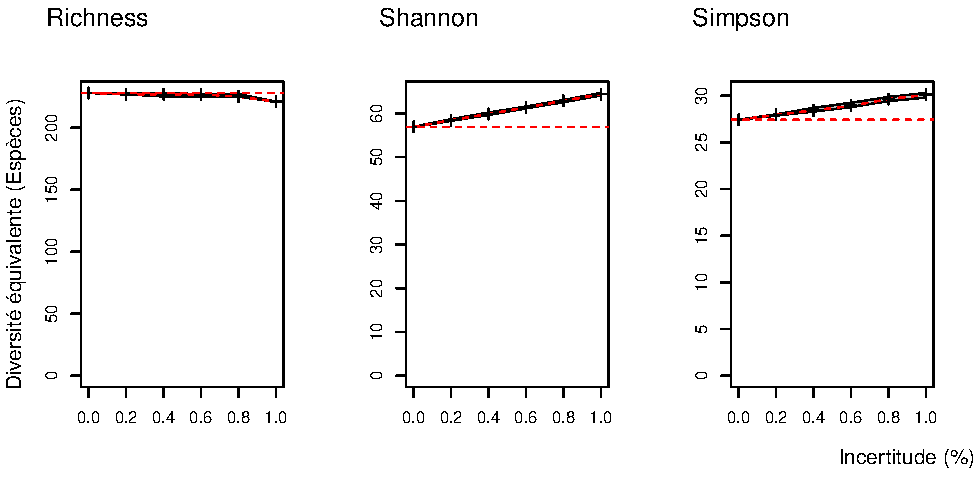
\includegraphics[width=1\linewidth]{MyBook_files/figure-latex/FigTreesSp-1} 

}

\caption{Profil de biais pour les diversité de Richesse, Shannon et Simpson au niveau spécifique le long d'un gradient d'indétermination correspondant au pourcentage d'individus identifiés uniquement par leur nom vernaculaire. Les profils de biais représentent la moyenne et les quantiles 0.025 et 0.975 de la distribution des diversités obtenues pour 100 simulations de tirage aléatoire et de propagation des incertitudes.}\label{fig:FigTreesSp}
\end{figure*}

Le profil de biais obtenu montre un effet non négligeable du degré
d'indétermination sur la mesure de la diversité. L'estimateur de la
richesse reste peu biaisé tant que le degré d'indétermination ne dépasse
pas 80\%, ce qui signifique que toutes les espèces sont représentées par
au moins un individu identifié au niveau botanique. En revanche les
diversités de Shannon et Simpson, et donc l'équitabilité des
communautés, sont significativement surestimées et ceci
proportionellement au degré d'indétermination.

La propagation des incertitudes tend donc à homogénéiser les abondances
de la communauté: les individus indéterminés tirés aléatoirement ont
plus de chances de orrespondre à une espèce abondante (par définition
plus fréquente) et d'être réattribuée par la méthode de propagation à
une espèce plus commune. Le biais semble donc difficile à formaliser car
il dépend de la relation entre rareté et probabilité d'indétermination
des espèces, qui est déterminée par la connaissances botaniques de
l'équipe d'identification.

Pour pallier ce biais nous avons choisis de nous rapporter au niveau
taxonomique supérieur et d'étudier la diversité des communautés en genre
botanique. Le biais de l'estimateur de diversité au niveau espèce est
bien moins important, ne dépassant pas 10\% de la diversité observée
\ref{fig:FigTreesGenus}. Par ailleurs, les estimateurs sont peu
variables et permettent de comparer correctement les communautés
communautés, pourvu que leurs degrés d'indétermination soient
similaires.

\begin{figure*}

{\centering 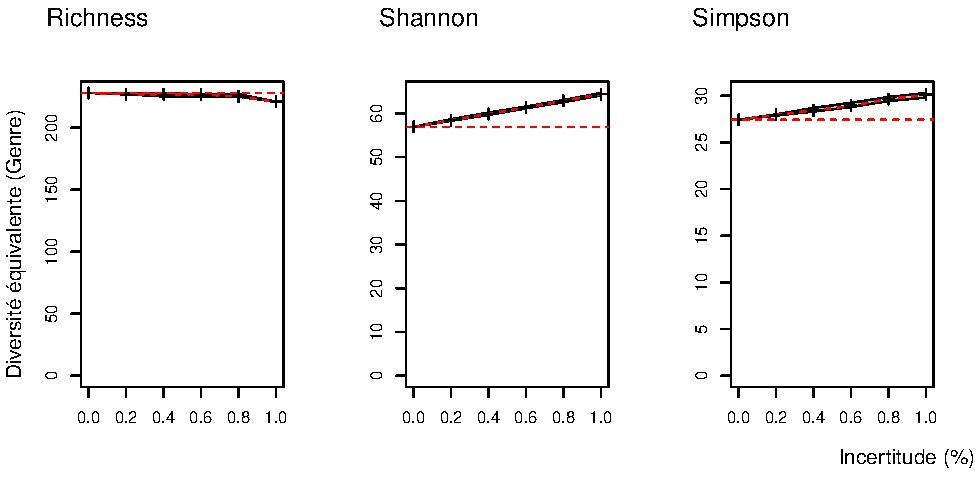
\includegraphics[width=0.6\linewidth]{MyBook_files/figure-latex/FigTreesGenus-1} 

}

\caption{Profil de biais pour les diversité de Richesse, Shannon et Simpson au niveau genre le long d'un gradient d'indétermination correspondant au pourcentage d'individus identifiés uniquement par leur nom vernaculaire. Les profils de biais représentent la moyenne et les quantiles 0.025 et 0.975 de la distribution des diversités obtenues pour 100 simulations de tirage aléatoire et de propagation des incertitudes.}\label{fig:FigTreesGenus}
\end{figure*}

\subsection{Cas particulier de
Paracou}\label{cas-particulier-de-paracou}

L'histoire de détermination botanique des parcelles de Paracou implique
une grande variabilité du degré d'indétermination au cours du temps et
des différences significatives entres les parcelles. Aujourd'hui tandis
que les parcelles contrôle et du traitement 3 sont bien déterminées,
moins de 5\% des arbres 'ne sont identifiés que par un nom
vernaculaire'ont pas d'identification botanique, d'autres parcelles du
traitement 1 ou 2 sont encore mal déterminées et pour certaines plus de
30\% des arbres n'ont pas d'identification botanique.

Jusqu'à présent le biais des estimateurs de diversité reste à resoudre,
en revanche il est possible de pallier ces différences de détermination
en considérant la compositon et la diversité des parcelles au niveau du
genre plutôt qu'au niveau de l'espèce.

\chapter{Article 2: trajectoires de diversité des
parcelles}\label{article-2-trajectoires-de-diversite-des-parcelles}

Nous proposons ici d'étudier sur 30 années la réponse des forêts
tropicales à un gradient de perturbation (10 à 60\% de biomasse
prélevée) et d'identifier les processus écologiques sous-jacents. Nous
avons analysé les trajectoires de composition, de richesse et
d'équitabilitét taxonomique et fonctionnelle et de redondance
fonctionnelle, en considérant 7 traits des feuilles, du bois et
d'histoire de vie représentatifs de l'écologie des espèces.

Les trajectoires de diversité ont démontré la restoration taxonomique
des communautés, maintenant leurs différences de composition initiales,
et leur restoration fonctionnelle selon une trajectoire rapide et
commune dans l'espace des traits. La théorie des perturbations
intermédiaires a démontré prédire correctement la trajectoire
fonctionnelle des communautés en fonction de l'intensité d'exploitation,
elle n'expliquait que médiocrement leurs trajectoires taxonomiques
troublées par une réorganisation de la redondance fonctionnelle et par
un recrutement des espèces rares inféodées aux forêts matures ralenti
par l'exclusion compétitive pour la lumière.

Bien que le fonctionnement des communautés soit restoré 30 ans après
perturbation leur composition et leur diversité en espèces rares restent
inachevées, altérant la structure taxonomique et la redondance
fonctionnelle de la communauté. Ces résultats soulignent d'une part la
nécessité d'adopter des cycles de régénération longs de plusieurs
décennies pour assurer une restoration complète des communautés, et
d'autre part interrogent la résilience des peuplements après plusieurs
perturbations.

\chapter{Article 3: Analyse du recrutement, support de la trajectoire
des
communautés}\label{article-3-analyse-du-recrutement-support-de-la-trajectoire-des-communautes}

La littérature récente en écologie tropicale a démontré l'implication de
processus déterministes et stochastiques dans la dynamique des
communautés mais leur signature structurelle sont difficilement
distinguables (Mouquet et Loreau
\protect\hyperlink{ref-Mouquet2003}{2003}; Chave
\protect\hyperlink{ref-Chave2004}{2004}). Nous proposons ici de
clarifier le rôle des processus écologiques régissant la réponse des
communautés en distinguant la trajectoire du recrutement de celles de la
communauté entière. Ces trajectoires de recrutement permettent d'une
part de distinguer les processus stochastiques et déterministes qui les
régissent, de spécifier les processus de compétition impliqués et de
déterminer la durée et l'intégralité de la résilience des communautés et
de leur fonctionnement.

Nous avons pour cela suivi pendant 30 ans les trajectoires de diversité
et de composition du recrutement dans 75 ha de forêts néotropicale
Amazonienne après un gradient de perturbation (de 15 à 60\% de la
biomasse prélevée). Nous avons analysé et comparé à des modèles nuls les
trajectoires de diversité et d'équitabilité taxonomique, de
renouvellement des espèces recrutées par rapport à la communauté
initiale avant perturbation, et de la diversité fonctionnelle (indice de
Rao) de 7 trais fonctionnels majeurs des feuilles, du bois et d'histoire
de vie.

Nous avons identifié trois phases de recrutement après perturbation,
définies par l'équilibre entre les processus déterministes et
stochastiques impliqués. Dans un premier temps les trajectoires sont
portées par la croissance de juvéniles recrutés aléatoirement dans la
communauté d'avant exploitation. Dans un deuxième temps les trajectoires
reposent sur les ``recrutés vrais'' issus de la banque de graines et
tributaires de processus d'exclusion pour la lumière favorisant les
espèces héliophiles à croissance rapide. La troisième et dernière phase
des trajectoires correspond au retour progressif vers un recrutement
aléatoire restorant la structure, la composition taxonomique et le
fonctionnement de la communauté initiale. Si le fontionnement du
recrutement a été rapidement retrouvé, la restoration taxonomique s'est
montrée longue, ce qui interroge l'intégralité de la résilience et
malgré la réelle restoration de la diversité et de la composition
initiale, Les différentes trajectoires ont par ailleurs confirmé une
restoration de la diversité fonctionnelle rapide mais plus lente de la
composition et de la diversité taxonomiques.

La trajectoire des communautés après perturbation résulte de la
combinaison des processus stochastiques, majeurs avant perturbation et
progressivement restorés par la suite, et de processus déterministes
d'exclusion compétitive favorisant les espèces héliophiles et à
croissance rapide. La résilience de la composition et la diversité
taxonomiques et fonctionnelles du recrutement a été confirmée mais
longue de plusieurs décennies, et confirme le risque de trajectoires
différentes dans le cas de perturbations répétées.

\chapter{Conclusion et perspectives}\label{conclusion-et-perspectives}

Au cours de cette thèse nous avons cherché à décrire et comprendre la
réponse aux perturbations des forêts tropicales pour pouvoir anticiper
leur devenir dans le contexte de changements actuel et affiner les
pratiques de gestion durable. Notre étude s'appuie largement sur les
données d'inventaire de Paracou, site expérimental idéal et unique
autant par la précision des inventaires que par la durée et la
régularité du suivi.

L'étude de la biodiversité est souvent limitée en temps, en espace et en
précision par le coût financier et humain des inventaires botaniques et
des bases de données fonctionnelles. Malgré leur qualité, les
inventaires de Paracou ne sont pas exempts de ces difficultés et le
premier travail de cette thèse a été de pallier les incertitudes des
inventaires et des bases de données fonctionnelles pour améliorer la
précision des estimateurs de diversité. Dans cette perspective
d'améliorer l'étude de la biodiversité avons appliqué l'estimateur de
diversité dans le cadre de l'exploitation forestière et proposons une
méthode d'inventaire permettant d'en optimiser la précision vis à vis du
suivi de la biodiversité.

Les contraintes méthodologiques résolues, nous avons étudié les
multiples aspects de la structure et de la trajectoire des forêts en
considérant la richesse, l'équitabilité et la composition des
communautés en espèces d'arbres (diversité taxonomique) et en
considérant leurs caractéristiques fonctionnelles d'acquisition des
ressources (diversité fonctionnelle). Les trajectoires de diversité ont
permis d'identifier la succession des processus écologiques déterminant
la réponse des communautés aux perturbations, que nous présenterons dans
une première. A la lumière de ces processus nous proposons ici une
discussion sur le maintien de l'intégrité et du fonctionnement des
écosystèmes forestiers dans le contexte de changements actuel et de la
possibilité d'une exploitation en forêt tropicale durable sur le long
terme.

\section{L'enfer vert, le déterminisme aléatoire (c'est n'importe quoi
comme
titre)}\label{lenfer-vert-le-determinisme-aleatoire-cest-nimporte-quoi-comme-titre}

Un débat fondamental de l'écologie est d'élucider les processus
régissant la coexistence des espèces et leur assemblage en communautés.
Spécifiquement le débat porte sur la validité de la théorie neutre qui
prédit un assemblage aléatoire des espèces, par rapport la théorie des
perturbations intermédiaires qui suppose l'existence de processus
déterministes sélectionnant les espèces selon leurs caractéristiques
fonctionnelles. L'implication de processus déterministes suppose la
convergence des trajectoires de diversité et de composition des
communautés vers leur état initial, déterminés par les caractéristiques
environnementales, et le maintien de leurs différences. La théorie
neutre à l'inverse suppose un assemblage des communautés dépend des
contingences historiques (arrivée d'espèces, mortalité aléatoire,
activité anthropique) ou géographiques (limitation de la dispersion) et
résulte en une dérive aléatoire des assemblages. Les deux théories
neutres et déterministes, qui se sont montrées pertinentes dans
différents cas de figure, ne sont cependant pas incompatibles. (Chave
\protect\hyperlink{ref-Chave2004}{2004}) propose une théorie intégrative
faisant intervenir les processus stochastiques comme les processus de
sélection déterministes dont les différentes combinaisons dans le temps
et l'espace expliquent la structure des communautés.

Dans cette étude nous avons pu décrire les trajectoires de diversité
taxonomique et fonctionnelle (en termes de stratégie d'acquisition de la
lumière) des communautés et en interpréter les processus sous-jacents.

\subsection{Trajectoires
fonctionnelles}\label{trajectoires-fonctionnelles}

La diversité et la composition fonctionnelles des communautés, qui
représentent directement le fonctionnement des écosystèmes, ont révélé
des trajectoires déterminée par la succession de différents processus de
sélection des espèces émergeants après perturbation. La réponse des
communautés dépend des changements biotiques et abiotiques qui accélère
la croissance des arbres et augmente le taux de recrutement. Les arbres
recrutés durant le 5 années suivant l'exploitation sont les juvéniles
déjà en place avant perturbation et qui réagissent les premiers aux
changements environnementaux. La diversité et la composition de ces
premiers recutés reproduit celle de la communauté avant perturbation et
aucun processus de sélection ne discrimine la croissance des espèces, si
bien que la première phase de recrutement avant perturbation ne modifie
pas le fonctionnement de la communauté. Dans un deuxième temps les
arbres recrutés sont issus de la germination des graines de la banque du
sol et soumis à l'exclusion compétitive pour la lumière. Les
trajectoires fonctionnelles sont alors déterminées par l'exclusion
d'espèces tolérantes à l'ombre, inféodées aux forêts non perturbées, en
faveur d'espèce pionnières à croissance rapide. La diversité
fonctionnelle du recrutement est restreinte aux stratégies d'acquisition
et d'utilisation de la lumière les plus efficaces, en particulier après
les perturbations les plus intenses qui entraînent une forte dominance
de quelques espèces très pionnières, telles que Cecropia spp.. Malgré
une diversité du recrutement plus faible, les principales espèces
recrutées étaient minoritaires avant perturbation si bien qu'à l'échelle
de la communauté entière l'équitabilité fonctionnelle augmente d'autant
plus que la perturbation est intense. Dans un troisième temps les
trajectoires révèlent un régime cyclique assurant la restoration des
conditions environnementales et du fonctionnement des communautés
initiales. Les processus de recrutment aléatoires propres aux
communautés non perturbées et ne favorisant pas les espèces pionnières
sont progressivement restaurés. Les trajectoires fonctionnelles
observées conforment la théorie des perturbations intermédiaires, qui
prédit une diversité élevée grâce à la variabilité dans le temps de
l'environnement et des processus de sélection compétitive qui en
résultent. Les trajectoires de diversité suivent un régime cyclique
assurant la résilience fonctionnelle des communautés par la restoration
de la diversité et de la composition et des processus de recrutement
initiaux. Trentes années ont quasiment permis la restoration du
fonctionnement des communautés et de la dynamique du recrutement, mais
l'impact de la perturbation sur la structure de redondance fonctionnelle
persiste. La redondance, qui quantifie les similarités fonctionnelles
entre espèces d'une communauté, n'a pas d'influence sur son
fonctionnement mais sur sa résilience. Après perturbation nous avons
observé une réorganisation de la redondance dans l'espace fonctionnel,
plus faible dans l'espace fonctionnel initial mais plus forte pour les
valeurs de traits d'acquisiton et d'utilisation efficaces des ressources
qui correspondent aux espèces pionnières recrutées en majorité. La
restauration de la structure de redondance fonctionnelle, inachevée 30
ans après exploitation, nuance l'intégralité de la résilience des
commmunautés.

\subsection{Trajectoires taxonomiques}\label{trajectoires-taxonomiques}

Les trajectoires fonctionnelles ont montré que la théorie des
perturbations intermédiaires était un bon modèle prédictif de la réponse
fonctionnelle des communautés aux perturbations, régie par l'émergence
de processus écologiques déterministes. La théories des perturbations
intermédiaires ne prédit que médiocrement les trajectoires taxonomiques,
perturbées et décorrélées des trajectoires fonctionnelles par le
difficile recrutement des espèces rares.

L'impact des perturbations sur la diversité taxonomique reste débattu et
une grande diversité de réponses a été observée selon l'échelle d'étude,
l'écosystème considéré et les modalités de la perturbation
({\textbf{???}}). Bien que les perturbations favorisent le recrutement
d'espèces auparavant peu communes, ce qui augmente la richesse et de
l'équitabilité de la communauté, les trajectoires taxonomiques varient
entre les communautés et sont peu corrélées à l'intensité de la
perturbation. Le schéma commun à toutes les communautés est en revanche
une restauration de la composition et la structure taxonomiques
initiales et donc à maintenir les différences de composition entre
communautés. Cette résilience signifie la convergence des communautés
vers une composition donnée, celle de la communauté avant perturbation,
et le maintien à long terme de plusieurs équilibres stables. La
compositon et la structure taxonomique initiales orientent donc les
trajectoire des communautés, ce qui explique leur forte variabilité. La
structure taxonomique des communautés restait après 30 ans plus impactée
par les perturbations que la structure fonctionnelle. Si les espèces
dominantes dans la communauté sont restaurées rapidement, déterminant la
restauration fonctionnelle de la communauté, la restoration des espèces
rares est plus lente et retarde les trajectoires taxonomiques par
rapport aux trajectoires fonctionnelles . La restauration des espèces
rares dépend de la structure de redondance fonctionnelle. La redondance
fonctionnelle, diminuée dans l'espace initial après exploitation, est
restaurée progressivement et avec elle les processus de compétition qui
limitent la similarité entre espèces. Les espèces rares manquant à la
restauration taxonomique sont des espèces inféodées aux communautés non
perturbées, fonctionnellement redondantes dans l'espace fonctionnel
initial et dont le recrutement est ralenti par la compétition.

La trajectoire taxonomique des communautés est donc déterminée par la
diversité et la composition de la communauté initiale et dépend de la
trajectoire de redondance fonctionnelle. Trente ans après exploitation,
la structure taxonomique reste impactées par la perturbation,ce qui
questionne sur l'intégralité de la résilience des communautés. Ces
modifications à long terme impliquent menacent de voir disparaître
certaines espèces rares et supposent une réponse différente des
communautés après de nouvelles perturbations.

\hypertarget{refs}{}
\hypertarget{ref-Asner2004}{}
Asner, Gregory P., Michael Keller, et Jose Natalino M Silva. 2004.
«~Spatial and temporal dynamics of forest canopy gaps following
selective logging in the eastern Amazon~». \emph{Global Change Biology}
10 (5): 765‑83.
doi:\href{https://doi.org/10.1111/j.1529-8817.2003.00756.x}{10.1111/j.1529-8817.2003.00756.x}.

\hypertarget{ref-Asner2009}{}
Asner, Gregory P., Thomas K. Rudel, T. Mitchell Aide, Ruth Defries, et
Ruth Emerson. 2009. «~A contemporary assessment of change in humid
tropical forests~». \emph{Conservation Biology} 23 (6): 1386‑95.
doi:\href{https://doi.org/10.1111/j.1523-1739.2009.01333.x}{10.1111/j.1523-1739.2009.01333.x}.

\hypertarget{ref-Baraloto2012}{}
Baraloto, Christopher, Quentin Molto, Suzanne Rabaud, Bruno Hérault,
Renato Valencia, Lilian Blanc, Paul V A Fine, et Jill Thompson. 2012.
«~Rapid Simultaneous Estimation of Aboveground Biomass and Tree
Diversity Across Neotropical Forests: A Comparison of Field Inventory
Methods ´~». \emph{Biotropica} 0 (0): 1‑11.

\hypertarget{ref-Begon2006}{}
Begon, Michael, Colin R Townsend, et John L Harper. 2006. \emph{Ecology:
from individuals to ecosystems}. Sirsi) i9781405111171.

\hypertarget{ref-Berry2008a}{}
Berry, Nicholas J., Oliver L. Phillips, Robert C. Ong, et Keith C.
Hamer. 2008. «~Impacts of selective logging on tree diversity across a
rainforest landscape: The importance of spatial scale~». \emph{Landscape
Ecology} 23 (8): 915‑29.
doi:\href{https://doi.org/10.1007/s10980-008-9248-1}{10.1007/s10980-008-9248-1}.

\hypertarget{ref-Cardinale2012}{}
Cardinale, Bradley J., J. Emmett Duffy, Andrew Gonzalez, David U.
Hooper, Charles Perrings, Patrick Venail, Anita Narwani, et al. 2012.
«~Biodiversity loss and its impact on humanity~». \emph{Nature} 489
(7415): 326‑26.
doi:\href{https://doi.org/10.1038/nature11373}{10.1038/nature11373}.

\hypertarget{ref-Carmona2016}{}
Carmona, Carlos P., Francesco de Bello, Norman W.H. Mason, et Jan Lepš.
2016. «~Traits Without Borders: Integrating Functional Diversity Across
Scales~». \emph{Trends in Ecology and Evolution} 31 (5): 382‑94.
doi:\href{https://doi.org/10.1016/j.tree.2016.02.003}{10.1016/j.tree.2016.02.003}.

\hypertarget{ref-Chao2015}{}
Chao, Anne, et Lou Jost. 2015. «~Estimating diversity and entropy
profiles via discovery rates of new species~». \emph{Methods in Ecology
and Evolution} 6 (8): 873‑82.
doi:\href{https://doi.org/10.1111/2041-210X.12349}{10.1111/2041-210X.12349}.

\hypertarget{ref-Chave2004}{}
Chave, J. 2004. «~Neutral theory and community ecology~». \emph{Ecology
Letters} 7 (3): 241‑53.
doi:\href{https://doi.org/10.1111/j.1461-0248.2003.00566.x}{10.1111/j.1461-0248.2003.00566.x}.

\hypertarget{ref-Chave2009}{}
Chave, Jerome, David Coomes, Steven Jansen, Simon L. Lewis, Nathan G.
Swenson, et Amy E. Zanne. 2009. «~Towards a worldwide wood economics
spectrum~». \emph{Ecology Letters} 12: 351‑66.
doi:\href{https://doi.org/10.1111/j.1461-0248.2009.01285.x}{10.1111/j.1461-0248.2009.01285.x}.

\hypertarget{ref-Chesson2000}{}
Chesson, Peter. 2000. «~Mechanisms of Maintenance of Species
Diversity~». \emph{Annual Review of Ecology and Systematics} 31: 343‑66.
doi:\href{https://doi.org/10.1146/annurev.ecolsys.31.1.343}{10.1146/annurev.ecolsys.31.1.343}.

\hypertarget{ref-CBDdiversity2011}{}
Convention on Biological Diversity, Secretariat of the, et Deutsche
Gesellschaft für Internationale Zusammenarbeit (giz) GmbH. 2011.
«~Biodiversity and Livelihoods REDD-plus Benefits~».

\hypertarget{ref-Dauby2012}{}
Dauby, Gilles, et Olivier J. Hardy. 2012. «~Sampled-based estimation of
diversity sensu stricto by transforming Hurlbert diversities into
effective number of species~». \emph{Ecography} 35 (7): 661‑72.
doi:\href{https://doi.org/10.1111/j.1600-0587.2011.06860.x}{10.1111/j.1600-0587.2011.06860.x}.

\hypertarget{ref-Denslow1998}{}
Denslow, Julie S, Aaron M Ellison, et Robert E Sanford. 1998. «~Treefall
gap size effects on above-and below-ground processes in a tropical wet
forest~». \emph{Journal of Ecology} 86 (4). Wiley Online Library:
597‑609.

\hypertarget{ref-Denslow1980}{}
Denslow, Julie Sloan. 1980. «~Gap Partitioning among Tropical Rainforest
Trees~». \emph{Biotropica} 12 (2): 47‑55.
doi:\href{https://doi.org/10.2307/2388156}{10.2307/2388156}.

\hypertarget{ref-Dirzo2003a}{}
Dirzo, R, et P H Raven. 2003. «~Global State of Biodiversity and Loss~».
\emph{Annual Review of Environment and Resources} 28 (1): 137‑67.
doi:\href{https://doi.org/10.1146/annurev.energy.28.050302.105532}{10.1146/annurev.energy.28.050302.105532}.

\hypertarget{ref-Elmqvist2003}{}
Elmqvist, T, C Folke, M Nystrom, G Peterson, J Bengtsson, B Walker, et J
Norberg. 2003. «~Response diversity, ecosystem change, and resilience~».
\emph{Frontiers in Ecology and the Environment} 1 (9): 488‑94.
doi:\href{https://doi.org/10.2307/3868116}{10.2307/3868116}.

\hypertarget{ref-FAO2009}{}
FAO. 2014a. «~Situation des Forêts du monde~». Rome: Organisation des
Nations Unies pour l'alimentation et l'agriculture.

\hypertarget{ref-FAO2014}{}
---------. 2014b. «~State of the World's Forests (SOFO)~». Rome: Food;
Agriculture Organization of the United Nations.

\hypertarget{ref-FAO2011}{}
FAO, ITTO. 2011. «~The state of forests in the Amazon Basin, Congo Basin
and Southest Asia~». Rome (italy).

\hypertarget{ref-Feeley2011}{}
Feeley, Kenneth J., et Miles R. Silman. 2011. «~The data void in
modeling current and future distributions of tropical species~».
\emph{Global Change Biology} 17 (1): 626‑30.
doi:\href{https://doi.org/10.1111/j.1365-2486.2010.02239.x}{10.1111/j.1365-2486.2010.02239.x}.

\hypertarget{ref-Ferry2010}{}
Ferry, Bruno, François Morneau, Jean Daniel Bontemps, Lilian Blanc, et
Vincent Freycon. 2010. «~Higher treefall rates on slopes and waterlogged
soils result in lower stand biomass and productivity in a tropical rain
forest~». \emph{Journal of Ecology} 98 (1): 106‑16.
doi:\href{https://doi.org/10.1111/j.1365-2745.2009.01604.x}{10.1111/j.1365-2745.2009.01604.x}.

\hypertarget{ref-Fisher1943}{}
Fisher, Author R a, a Steven Corbet, et C B Williams. 1943. «~The number
of animals in a random sample of an animal population~». \emph{Journal
of Animal Ecology} 12 (1): 42‑58.

\hypertarget{ref-FRA2000}{}
Forestry Department of the Food and Agriculture Organization of the
United Nations. 2000. «~Forest Resources Assessment 2000~».

\hypertarget{ref-FRA2015}{}
---------. 2015. «~Forest Resources Assessment 2015~». Food; Agriculture
Organization of the United Nations (FAO).

\hypertarget{ref-Funk2017}{}
Funk, Jennifer L., Julie E. Larson, Gregory M. Ames, Bradley J.
Butterfield, Jeannine Cavender-Bares, Jennifer Firn, Daniel C. Laughlin,
Ariana E. Sutton-Grier, Laura Williams, et Justin Wright. 2017.
«~Revisiting the Holy Grail: using plant functional traits to understand
ecological processes~». \emph{Biological Reviews} 92 (2): 1156‑73.
doi:\href{https://doi.org/10.1111/brv.12275}{10.1111/brv.12275}.

\hypertarget{ref-Gardner2007}{}
Gardner, Toby A., Jos Barlow, Luke W. Parry, et Carlos A. Peres. 2007.
«~Predicting the uncertain future of tropical forest species in a data
vacuum~». \emph{Biotropica} 39 (1): 25‑30.
doi:\href{https://doi.org/10.1111/j.1744-7429.2006.00228.x}{10.1111/j.1744-7429.2006.00228.x}.

\hypertarget{ref-Gentry1988}{}
Gentry, Alwyn H. 1988. «~Changes in Plant Community Diversity and
Floristic Composition on Environmental and Geographical Gradients~».
\emph{Annals of the Missouri Botanical Garden} 75 (1): 1‑34.

\hypertarget{ref-Good1953}{}
Good, I. J. 1953. «~The Population Frequency of Species and the
Estimation of Population Parameters~». \emph{Biometrika} 40 (3/4):
237‑64.

\hypertarget{ref-Goulamoussene2017}{}
Goulamoussène, Youven, Caroline Bedeau, Laurent Descroix, Laurent
Linguet, et Bruno Hérault. 2017. «~Environmental control of natural gap
size distribution in tropical forests~». \emph{Biogeosciences} 14 (2):
353‑64.
doi:\href{https://doi.org/10.5194/bg-14-353-2017}{10.5194/bg-14-353-2017}.

\hypertarget{ref-Grime1998}{}
Grime, JP. 1998. «~Benefits of plant diversity to ecosystems: immediate,
filter and founder effects~». \emph{Journal of Ecology} 86 (6). Wiley
Online Library: 902‑10.

\hypertarget{ref-Guitet2015}{}
Guitet, Stéphane, Raphaël Pélissier, Olivier Brunaux, Gaëlle Jaouen, et
Daniel Sabatier. 2015. «~Geomorphological landscape features explain
floristic patterns in French Guiana rainforest~». \emph{Biodiversity and
Conservation} 24 (5): 1215‑37.
doi:\href{https://doi.org/10.1007/s10531-014-0854-8}{10.1007/s10531-014-0854-8}.

\hypertarget{ref-Guitet2017}{}
Guitet, Stéphane, Daniel Sabatier, Olivier Brunaux, Pierre Couteron,
Thomas Denis, Vincent Freycon, Sophie Gonzalez, et al. 2017.
«~Disturbance regimes drive the diversity of regional floristic pools
across Guianan rainsforest landscapes~». \emph{Scientific Reports}
Submitted (December 2016): 1‑12.
doi:\href{https://doi.org/10.1038/s41598-018-22209-9}{10.1038/s41598-018-22209-9}.

\hypertarget{ref-Guitet2014}{}
Guitet, Stéphane, Daniel Sabatier, Olivier Brunaux, Bruno Hérault,
Mélaine Aubry-Kientz, Jean-François François Molino, et Christopher
Baraloto. 2014. «~Estimating tropical tree diversity indices from
forestry surveys: A method to integrate taxonomic uncertainty~».
\emph{Forest Ecology and Management} 328: 270‑81.
doi:\href{https://doi.org/10.1016/j.foreco.2014.05.045}{10.1016/j.foreco.2014.05.045}.

\hypertarget{ref-Hansen2013}{}
Hansen, Matthew C, Peter V Potapov, Rebecca Moore, Matt Hancher, SAa
Turubanova, Alexandra Tyukavina, David Thau, et al. 2013.
«~High-resolution global maps of 21st-century forest cover change~».
\emph{science} 342 (6160). American Association for the Advancement of
Science: 850‑53.

\hypertarget{ref-Herault2011}{}
Hérault, Bruno, Bénédicte Bachelot, Lourens Poorter, Vivien Rossi, Frans
Bongers, Jérôme Chave, C. E Timothy Paine, Fabien Wagner, et Christopher
Baraloto. 2011. «~Functional traits shape ontogenetic growth
trajectories of rain forest tree species~». \emph{Journal of Ecology}
99: 1431‑40.
doi:\href{https://doi.org/10.1111/j.1365-2745.2011.01883.x}{10.1111/j.1365-2745.2011.01883.x}.

\hypertarget{ref-Hill1973}{}
Hill, M. O. 1973. «~Diversity and Evenness : A Unifying Notation and Its
Consequences~». \emph{Ecological Society of America} 54 (2): 427‑32.

\hypertarget{ref-Hubbell2001}{}
Hubbell, Stephen P. 2001. \emph{The Unified Neutral Theory of
Biodiversity and Biogeography}. Princeton University Press.

\hypertarget{ref-Isbell2017}{}
Isbell, Forest, Andrew Gonzalez, Michel Loreau, Jane Cowles, Sandra
Díaz, Andy Hector, Georgina M. MacE, et al. 2017. «~Linking the
influence and dependence of people on biodiversity across scales~».
\emph{Nature} 546 (7656): 65‑72.
doi:\href{https://doi.org/10.1038/nature22899}{10.1038/nature22899}.

\hypertarget{ref-Jones1994}{}
Jones, Clive G, John H Lawton, et Moshe Shachak. 1994. «~Organisms as
ecosystem engineers~». In \emph{Ecosystem management}, 130‑47. Springer.

\hypertarget{ref-Kariuki2006a}{}
Kariuki, Maina, Robert M. Kooyman, R. G B Smith, Grant Wardell-Johnson,
et Jerome K. Vanclay. 2006. «~Regeneration changes in tree species
abundance, diversity and structure in logged and unlogged subtropical
rainforest over a 36-year period~». \emph{Forest Ecology and Management}
236 (2-3): 162‑76.
doi:\href{https://doi.org/10.1016/j.foreco.2006.09.021}{10.1016/j.foreco.2006.09.021}.

\hypertarget{ref-Kattge2011}{}
Kattge, J., S. Díaz, S. Lavorel, I. C. Prentice, P. Leadley, G. Bönisch,
E. Garnier, et al. 2011. «~TRY - a global database of plant traits~».
\emph{Global Change Biology} 17 (9): 2905‑35.
doi:\href{https://doi.org/10.1111/j.1365-2486.2011.02451.x}{10.1111/j.1365-2486.2011.02451.x}.

\hypertarget{ref-Kunstler2012}{}
Kunstler, Georges, Sébastien Lavergne, Benoît Courbaud, Wilfried
Thuiller, Ghislain Vieilledent, Niklaus E. Zimmermann, Jens Kattge, et
David A. Coomes. 2012. «~Competitive interactions between forest trees
are driven by species' trait hierarchy, not phylogenetic or functional
similarity: Implications for forest community assembly~». \emph{Ecology
Letters} 15 (8): 831‑40.
doi:\href{https://doi.org/10.1111/j.1461-0248.2012.01803.x}{10.1111/j.1461-0248.2012.01803.x}.

\hypertarget{ref-Loreau2005}{}
Loreau, M. 2005. «~Actes de la Conférence Internationale Biodiversité,
Science et Gouvernance~». In \emph{Discours de Clôture}, 254‑56. IRD
Editions.

\hypertarget{ref-Magurran2004}{}
Magurran, A E. 2004. \emph{Measuring Biological Diversity}. Blackwell
Science Ltd.

\hypertarget{ref-Magurran1988}{}
Magurran, Anne E. 1988. \emph{Ecological diversity and its measurement}.
NJ, Prince. Princeton.

\hypertarget{ref-Malhi2008}{}
Malhi, Yadvinder, J Timmons Roberts, Richard A Betts, Timothy J Killeen,
Wenhong Li, et Carlos A Nobre. 2008. «~Climate change, deforestation,
and the fate of the Amazon~». \emph{science} 319 (5860). American
Association for the Advancement of Science: 169‑72.

\hypertarget{ref-Marcon2015b}{}
Marcon, Eric. 2015. «~Practical Estimation of Diversity from Abundance
Data~». \emph{HAL archives-ouvertes}, 9.

\hypertarget{ref-McGill2007}{}
McGill, B. J., R. S. Etienne, J. S. Gray, D. Alonso, M. J. Anderson, H.
Kassa Benecha, M. Dornelas, et al. 2007. «~Species abundance
distributions : moving beyond single prediction theories to integration
within an ecological framework~». \emph{Ecology Letters} 10: 995‑1015.
doi:\href{https://doi.org/10.1111/j.1461-0248.2007.01094.x}{10.1111/j.1461-0248.2007.01094.x}.

\hypertarget{ref-McGill2006}{}
McGill, Brian J., Brian J. Enquist, Evan Weiher, et Mark Westoby. 2006.
«~Rebuilding community ecology from functional traits~». \emph{Trends in
Ecology and Evolution} 21 (4): 178‑85.
doi:\href{https://doi.org/10.1016/j.tree.2006.02.002}{10.1016/j.tree.2006.02.002}.

\hypertarget{ref-Mendes2008}{}
Mendes, Renio S, Luiz R Evangelista, Sidinei M Thomaz, et Angelo A
Agostinho. 2008. «~A unifed index to measure ecological diversity and
species rarity~». \emph{Ecography} 31 (February): 450‑56.
doi:\href{https://doi.org/10.1111/j.2008.0906-7590.05469.x}{10.1111/j.2008.0906-7590.05469.x}.

\hypertarget{ref-Mittermeier2003}{}
Mittermeier, R. A., C. G. Mittermeier, T. M. Brooks, J. D. Pilgrim, W.
R. Konstant, G. A. B. da Fonseca, et C. Kormos. 2003. «~Wilderness and
biodiversity conservation~». \emph{Proceedings of the National Academy
of Sciences} 100 (18): 10309‑13.
doi:\href{https://doi.org/10.1073/pnas.1732458100}{10.1073/pnas.1732458100}.

\hypertarget{ref-Molino2001}{}
Molino, J F, et Daniel Sabatier. 2001. «~Tree diversity in tropical rain
forests: a validation of the intermediate disturbance hypothesis.~»
\emph{Science (New York, N.Y.)} 294 (5547): 1702‑4.
doi:\href{https://doi.org/10.1126/science.1060284}{10.1126/science.1060284}.

\hypertarget{ref-Morales-Hidalgo2015}{}
Morales-Hidalgo, David, Sonja N. Oswalt, et E. Somanathan. 2015.
«~Status and trends in global primary forest, protected areas, and areas
designated for conservation of biodiversity from the Global Forest
Resources Assessment 2015~». \emph{Forest Ecology and Management} 352.
Elsevier B.V.: 68‑77.
doi:\href{https://doi.org/10.1016/j.foreco.2015.06.011}{10.1016/j.foreco.2015.06.011}.

\hypertarget{ref-Motomura1932}{}
Motomura, I. 1932. «~On the statistical treatment of communities~».
\emph{Zoological Magazine} 44: 379‑83.

\hypertarget{ref-Mouillot2013a}{}
Mouillot, David, Nicholas A J Graham, Sébastien Villéger, Norman W H
Mason, et David R. Bellwood. 2013. «~A functional approach reveals
community responses to disturbances~». \emph{Trends in Ecology and
Evolution} 28 (3): 167‑77.
doi:\href{https://doi.org/10.1016/j.tree.2012.10.004}{10.1016/j.tree.2012.10.004}.

\hypertarget{ref-Mouquet2003}{}
Mouquet, Nicolas, et Michel Loreau. 2003. «~Community patterns in
source-sink metacommunities~». \emph{The american naturalist} 162 (5).
The University of Chicago Press: 544‑57.

\hypertarget{ref-Myers2000}{}
Myers, Norman, Russell A. Mittermeier, Cristina G. Mittermeier, Gustavo
A. B. da Fonseca, et Jennifer Kent. 2000. «~Biodiversity hotspots for
conservation priorities~». \emph{Nature} 403 (6772): 853‑58.
doi:\href{https://doi.org/10.1038/35002501}{10.1038/35002501}.

\hypertarget{ref-DeNoter2008}{}
Noter, C. de. 2008. «~Etat des connaissances, analyse et synthèse
bibliographique sur la faune de Guyane en vue d'étudier les
potentialités de développement économique et de transfert de
technologies.~» DRRT Guyane.

\hypertarget{ref-Oldeman1968}{}
Oldeman, Roelof A. A. 1968. «~Sur la valeur des noms vernaculaires des
plantes en Guyane Francaise~».

\hypertarget{ref-Otani2018}{}
Otani, Tatsuya, Adriano J.N. Lima, Rempei Suwa, Marcio R.M. Amaral,
Shinta Ohashi, Alberto C.M. Pinto, Joaquim Dos Santos, Takuya Kajimoto,
Niro Higuchi, et Moriyoshi Ishizuka. 2018. «~Recovery of above-ground
tree biomass after moderate selective logging in a central Amazonian
forest~». \emph{IForest} 11 (3): 352‑59.
doi:\href{https://doi.org/10.3832/ifor2534-011}{10.3832/ifor2534-011}.

\hypertarget{ref-Pachauri2014}{}
Pachauri, R, et L Meyer. 2014. «~Climate change 2014: Synthesis report.
fifth assessment report of the intergovernmental panel on climate
change~». \emph{Tech. Rep.} IPCC.

\hypertarget{ref-Pan2011}{}
Pan, Yude, Richard A Birdsey, Jingyun Fang, Richard Houghton, Pekka E
Kauppi, Werner A Kurz, Oliver L Phillips, et al. 2011. «~A large and
persistent carbon sink in the world's forests~». \emph{Science}.
American Association for the Advancement of Science, 1201609.

\hypertarget{ref-Patil1982}{}
Patil, G.P., et Taillie C. 1982. «~Diversity as a concept and its
measuremente: Rejoinder~».

\hypertarget{ref-Perez-Harguindeguy2013}{}
Pérez-Harguindeguy, N., S. Díaz, E. Garnier, S. Lavorel, H. Poorter, P.
Jaureguiberry, M. S. Bret-Harte, et al. 2013. «~New handbook for
standardised measurement of plant functional traits worldwide~».
\emph{Australian Journal of Botany} 61: 167‑234.
doi:\href{https://doi.org/10.1071/BT12225}{10.1071/BT12225}.

\hypertarget{ref-Podani2013}{}
Podani, János, Carlo Ricotta, et Dénes Schmera. 2013. «~A general
framework for analyzing beta diversity, nestedness and related
community-level phenomena based on abundance data~». \emph{Ecological
Complexity} 15: 52‑61.
doi:\href{https://doi.org/10.1016/j.ecocom.2013.03.002}{10.1016/j.ecocom.2013.03.002}.

\hypertarget{ref-Power1996}{}
Power, Mary E, David Tilman, James A Estes, Bruce A Menge, William J
Bond, Scott Mills, Gretchen Daily, et al. 1996. «~Challenges in the
Quest for Keystones~». \emph{Bioscience} 46 (8): 609‑20.
doi:\href{https://doi.org/10.2307/1312990}{10.2307/1312990}.

\hypertarget{ref-Purvis2000}{}
Purvis, Andy, et Andy Hector. 2000. «~Getting the measure of
biodiversity~». \emph{Nature Insight Biodiverstiy} 405 (6783): vol 405
no. 6783. doi:\href{https://doi.org/10.1038/35012221}{10.1038/35012221}.

\hypertarget{ref-Reich1997}{}
Reich, Peter B, Michael B Walters, et David S Ellsworth. 1997. «~From
tropics to tundra: Global convergence in plant functioning~».
\emph{Ecology} 94 (December): 13730‑4.
doi:\href{https://doi.org/10.1073/pnas.94.25.13730}{10.1073/pnas.94.25.13730}.

\hypertarget{ref-Reich2014}{}
Reich, Peter B. 2014. «~The world-wide 'fast-slow' plant economics
spectrum: A traits manifesto~». \emph{Journal of Ecology} 102: 275‑301.
doi:\href{https://doi.org/10.1111/1365-2745.12211}{10.1111/1365-2745.12211}.

\hypertarget{ref-Robert2003}{}
Robert, A., et M. A. Moravie. 2003. «~Topographic variation and stand
heterogeneity in a wet evergreen forest in India~». \emph{Journal of
Tropical Ecology} 19: 697‑707.

\hypertarget{ref-Roy2017}{}
Roy, David P, et Sanath Sathyachandran Kumar. 2017. «~Multi-year MODIS
active fire type classification over the Brazilian Tropical Moist Forest
Biome~». \emph{International Journal of Digital Earth} 10 (1). Taylor \&
Francis: 54‑84.

\hypertarget{ref-Sabatier1989}{}
Sabatier, Daniel, et Marie-Françoise Prévost. 1989. «~Quelques données
sur la composition floristique et la diversité des peuplements
forestiers~». \emph{BOIS \& FORETS DES TROPIQUES} 219 (219): 31‑55.

\hypertarget{ref-Sabatier1997}{}
Sabatier, Daniel, Michel Grimaldi, Marie-Françoise Prévost, J.
Guillaume, M. Gordon, M. Dosso, et P. Curmi. 1997. «~The influence of
soil cover organization on the floristic and structural heterogeneity of
a Guianan rain forest~». \emph{Plant Ecology} 131 (1): 81‑108.

\hypertarget{ref-Sakschewski2016}{}
Sakschewski, Boris, Werner von Bloh, Alice Boit, Lourens Poorter,
Marielos Peña-Claros, Jens Heinke, Jasmin Joshi, et Kirsten Thonicke.
2016. «~Resilience of Amazon forests emerges from plant trait
diversity~». \emph{Nature Climate Change} 1 (August).
doi:\href{https://doi.org/10.1038/nclimate3109}{10.1038/nclimate3109}.

\hypertarget{ref-Scheiter2013}{}
Scheiter, Simon, Liam Langan, et Steven I Higgins. 2013.
«~Next-generation dynamic global vegetation models: learning from
community ecology~». \emph{The New phytologist} 198 (3): 957‑69.
doi:\href{https://doi.org/10.1111/nph.12210}{10.1111/nph.12210}.

\hypertarget{ref-Schlaepfer2000}{}
Schlaepfer, Rodolphe, et Chris Elliott. 2000. «~Ecological and landscape
considerations in forest management: the end of forestry?~» In
\emph{Sustainable forest management}, 1‑67. Springer.

\hypertarget{ref-Schnitzer2001}{}
Schnitzer, Stefan A, et Walter P Carson. 2001. «~Treefall Gaps and the
Maintenance of Species Diversity in a Tropical Forest~». \emph{Ecology}
82 (4): 913‑19.

\hypertarget{ref-Shannon1948}{}
Shannon, C. E. 1948. «~A Mathematical Theory of Communication~».
\emph{The Bell System Technical Journal} 27 (379-423): 623‑56.

\hypertarget{ref-Sheil2003}{}
Sheil, Douglas, et David F.R.P. Burslem. 2003. «~Disturbing hypotheses
in tropical forests~». \emph{Trends in Ecology and Evolution} 18 (1):
18‑26.
doi:\href{https://doi.org/10.1016/S0169-5347(02)00005-8}{10.1016/S0169-5347(02)00005-8}.

\hypertarget{ref-Silvertown2004}{}
Silvertown, Jonathan. 2004. «~Plant coexistence and the niche~».
\emph{Trends in Ecology \& Evolution} 19 (11). Elsevier: 605‑11.

\hypertarget{ref-Simpson1949}{}
Simpson, E. H. 1949. «~Measurement of Diversity~». \emph{Nature} 163
(4148): 688.

\hypertarget{ref-Summit1992}{}
Summit, Earth. 1992. «~Agenda 21~». \emph{The United Nations programme
for action from Rio}.

\hypertarget{ref-terSteege2006}{}
Ter Steege, Hans, Nigel CA Pitman, Oliver L Phillips, Jerome Chave,
Daniel Sabatier, Alvaro Duque, Jean-François Molino, et al. 2006.
«~Continental-scale patterns of canopy tree composition and function
across Amazonia~». \emph{Nature} 443 (7110). Nature Publishing Group:
444.

\hypertarget{ref-terSteege2000}{}
Ter Steege, Hans, Daniel Sabatier, Hernán Castellanos, Tinde Van Andel,
Joost Duivenvoorden, Alexandre Adalardo De Oliveira, Renske Ek, Ramesh
Lilwah, Paul Maas, et Scott Mori. 2000. «~An analysis of the floristic
composition and diversity of Amazonian forest including those of the
Guiana Shield~». \emph{Journal of Tropical Ecology} 16 (6).
AgroParisTech: 801‑28.
doi:\href{https://doi.org/10.1017/S0266467400001735}{10.1017/S0266467400001735}.

\hypertarget{ref-Tilman2014}{}
Tilman, David, Forest Isbell, et Jane M. Cowles. 2014. «~Biodiversity
and Ecosystem Functioning~». \emph{Annual Review of Ecology, Evolution,
and Systematics} 45 (1): 471‑93.
doi:\href{https://doi.org/10.1146/annurev-ecolsys-120213-091917}{10.1146/annurev-ecolsys-120213-091917}.

\hypertarget{ref-Tokeshi1993}{}
Tokeshi, Mutsunori. 1993. «~Species Abundance Patterns and Community
Structure~». \emph{Advances in Ecological Research, Vol 24} 24: 111‑86.

\hypertarget{ref-Tothmeresz1995}{}
Tothmeresz, Béla, et Béla Tóthmérész. 1995. «~Comparison of different
methods for diversity ordering~». \emph{Journal of Vegetation Science} 6
(2): 283‑90.
doi:\href{https://doi.org/10.2307/3236223}{10.2307/3236223}.

\hypertarget{ref-Valverde-Barrantes2017}{}
Valverde-Barrantes, Oscar J., Grégoire T. Freschet, Catherine Roumet, et
Christopher B. Blackwood. 2017. «~A worldview of root traits: the
influence of ancestry, growth form, climate and mycorrhizal association
on the functional trait variation of fine-root tissues in seed plants~».
\emph{New Phytologist}.
doi:\href{https://doi.org/10.1111/nph.14571}{10.1111/nph.14571}.

\hypertarget{ref-Violle2007b}{}
Violle, Cyrille, Marie-Laure Laure Navas, Denis Vile, Elena Kazakou,
Claire Fortunel, Irène Hummel, et Eric Garnier. 2007. «~Let the concept
of trait be functional!~» \emph{Oikos} 116 (5): 882‑92.
doi:\href{https://doi.org/10.1111/j.2007.0030-1299.15559.x}{10.1111/j.2007.0030-1299.15559.x}.

\hypertarget{ref-Vitousek1997}{}
Vitousek, Peter M, Harold A Mooney, Jane Lubchenco, et Jerry M Melillo.
1997. «~Human domination of Earth's ecosystems~». \emph{Science} 277
(5325). American Association for the Advancement of Science: 494‑99.

\hypertarget{ref-Wagner2011}{}
Wagner, Fabien, Bruno Hérault, Clément Stahl, Damien Bonal, et Vivien
Rossi. 2011. «~Modeling water availability for trees in tropical
forests~». \emph{Agricultural and Forest Meteorology} 151 (9). Elsevier
B.V.: 1202‑13.
doi:\href{https://doi.org/10.1016/j.agrformet.2011.04.012}{10.1016/j.agrformet.2011.04.012}.

\hypertarget{ref-Westoby1998}{}
Westoby, Mark. 1998. «~A leaf-height-seed (LHS) plant ecology strategy
scheme~». \emph{Plant and Soil} 199: 213‑27.
doi:\href{https://doi.org/10.1023/A:1004327224729}{10.1023/A:1004327224729}.

\hypertarget{ref-Whittaker1965}{}
Whittaker, R. H. 1965. «~Dominance and diversity in land plant
communities: numerical relations of species express the importance of
competition in community function and evolution~». \emph{Science} 147
(3655): 250‑60.

\hypertarget{ref-Wright2004}{}
Wright, Ian J., Peter B. Reich, Mark Westoby, David D. Ackerly, Zdravko
Baruch, Frans Bongers, Jeannine Cavender-Bares, et al. 2004. «~The
worldwide leaf economics spectrum~». \emph{Nature} 428 (6985): 821‑27.
doi:\href{https://doi.org/10.1038/nature02403}{10.1038/nature02403}.


\end{document}
